%%%%%%%%%%%%%%%%%%%%%%%%%%%%%%%%%%%%%%%%%%%%%%%%%%%%%%%%%%%%%%%%%%%%%%%%%%%%%%%%
%2345678901234567890123456789012345678901234567890123456789012345678901234567890
%        1         2         3         4         5         6         7         8

\documentclass[letterpaper, 10 pt, conference]{ieeeconf}  % Comment this line out
                                                          % if you need a4paper
%\documentclass[a4paper, 10pt, conference]{ieeeconf}      % Use this line for a4
                                                          % paper

\IEEEoverridecommandlockouts                              % This command is only
                                                          % needed if you want to
                                                          % use the \thanks command
\overrideIEEEmargins
% See the \addtolength command later in the file to balance the column lengths
% on the last page of the document



% The following packages can be found on http:\\www.ctan.org
\usepackage{graphics} % for pdf, bitmapped graphics files
\usepackage{epsfig} % for postscript graphics files
 \usepackage{mathptmx} % assumes new font selection scheme installed
% \usepackage{times} % assumes new font selection scheme installed
\usepackage{amsmath} % assumes amsmath package installed
\usepackage{amssymb}  % assumes amsmath package installed
\usepackage{subfigure}
\usepackage{xcolor}

\newcommand{\usequence}[2]{(u_{i,t})_{i=1,t=1}^{#1,#2}}
\newcommand{\contTilde}[1]{\mathbf{\tilde{#1}}}
\newcommand{\transpose}{\mathsf{T}}
\newcommand{\myinner}[1]{\langle(#1)x,x\rangle}
\newcommand{\quadinner}[1]{x^{\transpose}(#1)x}
\DeclareMathOperator{\contB}{\mathbf{B}}
\DeclareMathOperator{\Log}{\mathrm{Log}}
\newcommand{\BK}[1]{\mathbf{B}\bar{K}_{#1}}
%bound \| x_t - x_{t|t} \|
\newcommand{\boundxtxtgt}[2]{C_{fb}^{2}\|\bar{x}_{1}\|[\frac{C_{K}}{\gamma-1}\bigg(\frac{1-(\eta\gamma)^{#1}}{1-\eta\gamma} - \frac{1-\eta^{#1}}{1-\eta} \bigg){#2}+\varepsilon_{K}\bigg(\frac{(#1-1)\eta^{#1+1}-#1\eta^{#1}+\eta}{(1-\eta)^{2}}\bigg)]}
\DeclareMathOperator{\tempRBP}{R + B^{\transpose}PB}

% \newcommand{\boundxtxtgt1}[1]{\frac{#1}{2}}
%bound |K_t|t - K_t^*|
\newcommand{\boundKt}{C_{K^{'}}\gamma^{W-1} + \gamma_{K^{'}}}

%bound xt|t
\newcommand{\boundxtgt}[1]{C_{fb}\eta^{#1}}

% \newcommand{\\det}{\mathit{\det}}
% \newcommand{\Log}[1]{\text{Log}}

\newtheorem{problem}{Problem}
\newtheorem{lemma}{Lemma}
\newtheorem{assumption}{Assumption}
\newtheorem{definition}{Definition}
\newtheorem{corollary}{Corollary}
\newtheorem{proposition}{Proposition}
\newtheorem{remark}{Remark}
\newtheorem{theorem}{Theorem}

\title{\LARGE \bf
Online Linear-Quadratic Feedback Potential Dynamic Games:\\ An Algorithm and Regret Analysis
}

%\author{ \parbox{3 in}{\centering Huibert Kwakernaak*
%         \thanks{*Use the $\backslash$thanks command to put information here}\\
%         Faculty of Electrical Engineering, Mathematics and Computer Science\\
%         University of Twente\\
%         7500 AE Enschede, The Netherlands\\
%         {\tt\small h.kwakernaak@autsubmit.com}}
%         \hspace*{ 0.5 in}
%         \parbox{3 in}{ \centering Pradeep Misra**
%         \thanks{**The footnote marks may be inserted manually}\\
%        Department of Electrical Engineering \\
%         Wright State University\\
%         Dayton, OH 45435, USA\\
%         {\tt\small pmisra@cs.wright.edu}}
%}

\author{Yitian Chen, Timothy Molloy, Iman Shames% <-this % stops a space
}
\allowdisplaybreaks


\begin{document}



\maketitle
\thispagestyle{empty}
\pagestyle{empty}

%%%%%%%%%%%%%%%%%%%%%%%%%%%%%%%%%%%%%%%%%%%%%%%%%%%%%%%%%%%%%%%%%%%%%%%%%%%%%%%%
\begin{abstract}
In this paper, we propose and analyse a new method for online feedback potential dynamic game for linear system dynamics and time-varying quadratic costs. The cost matrices are revealed sequentially for each player with the potential for future values to be previewed over a short window. Our novel method involves using the available cost matrices to predict the optimal trajectory, and a tracking controller to drive the system towards it. We adopted the notion of \emph{dynamic social regret} to measure the performance of this proposed method for the online feedback potential dynamic game, with our main result being that the \emph{dynamic social regret} of our method is upper bounded by a constant. Moreover, the regret is upperbounded by a sum of two terms. One decays exponentially as the preview horizon grows, while the other depends on the distance between cost matrices for each player at each time step. In our simulations, we demonstrate that the \emph{dynamic social regret} for our method stabilizes at a constant level as the time horizon grows while also showing a faster-than-exponential decay as the preview window length increases when the time step is fixed.
\end{abstract}


%%%%%%%%%%%%%%%%%%%%%%%%%%%%%%%%%%%%%%%%%%%%%%%%%%%%%%%%%%%%%%%%%%%%%%%%%%%%%%%%
\section{INTRODUCTION}
% \begin{enumerate}
%     \item Introduce Dynamic games
%     \item potential examples of online dynamic game
%     \item Introduce optimal control online
% \end{enumerate}

Game theory is a mathematical discipline that explores the dynamics of decision-making among rational players. It has proven invaluable in modelling complex scenarios involving multiple agents, such as optimizing network resources in contexts like multichannel communication and resource allocation. These situations often feature interdependent strategies where one decision-maker's choices can influence others.

In noncooperative dynamic games, participants engage in competitive interactions within a continually changing environment. This environment can be captured by a deterministic dynamical system, comprising a set of states and a state-transition equation. Each player incurs time-varying costs that hinge on both the present state and the decisions of all participants.

To illustrate, consider the example of food delivery from distributors to grocery stores. The state at any given time encapsulates information about inventory levels at a distributor warehouse. Meanwhile, the decisions involve determining how much food each distributor (indexed as $i$) should dispatch to the stores. These decisions come with associated costs, for instance, profit and product availability are contingent on the states and choices made.

However, real-world complexity often limits access to comprehensive future profit and product availability data for specific goods. Therefore, we cannot assume we have access to full information for all costs over a given period. In this context, we frame the problem as a dynamic game. At each time step, a player makes a decision based on the available cost information that can be accessed. This setup is referred to as an online dynamic game. The performance of each player is gauged by quantifying the discrepancy between the current decision and its Nash Equilibrium when all cost information is revealed to all players. In the Nash Equilibrium, each player's strategy is optimal when considering the decisions of other players. This paper aims at identifying the classes of dynamic games, referred to as \emph{potential dynamic games}, where the Nash Equilibrium can be obtained by solving a single optimal control problem.

To the best of our knowledge, there has been no work on this online dynamic game problem. A related concept is the online optimal control problem, which has been extensively studied in literature such as \cite{zhang_regret_2021}, \cite{chen_regret_2023} and \cite{cohen_online_2018}. However, it's important to note that in the online optimal control problem, only one player is involved in the dynamic game. Under certain conditions pertaining to system dynamics and cost functions, the optimal solution aligns with the concept of a feedback Nash equilibrium. Consequently, the online dynamic game problem can be seen as a natural extension of the online optimal control problem, introducing multiple players into the dynamic interaction.

The key contributions of this paper are:
\begin{enumerate}
    \item The formulation of a novel online feedback potential dynamic game problem with a dynamic social regret performance measure;
    \item An algorithm based on predicting and tracking a feedback Nash equilibrium;
    \item An upper bound on the regret achieved by our proposed algorithm.
\end{enumerate}
% There are similar results and algorithms that are available for online LQ optimal control problems \cite{chen_regret_2023},\cite{zhang_regret_2021}. However, to the best of our knowledge, they had not been extended to online dynamic games. We use the notion of \emph{dynamic social regret} to capture the discrepancy between the decisions made by players without accessing full information from the future and their Nash equilibrium solution in hindsight.

% {\color{red} Yitian todo: two-three sentences explaining that whilst similar results and algorithms are avaiable for online LQ optimal control problems, they have not been extended to dynamics games. Explain also importance of dynamic social regret providing an aggregate performance measure.
% }


This paper is structured as follows.
In Section \ref{sec:problem_formulation}, we formulate our online feedback potential game problem. In Section \ref{sec:approach}, we present our proposed algorithm to solve the online feedback potential game problem and the upperbound of its performance that is measured by \emph{dynamic social regret}. In Section \ref{sec:numerical}, we show numerical examples to demonstrate the performance of the proposed algorithm based on the example of the network flow control problem. Lastly, we make our conclusions and discuss possible future directions in Section \ref{sec:conclusions}.

\emph{Notation:}
For a matrix $\mathbf{H}$ with 2 row partitions and 2 column partitions, i.e.,
    $\mathbf{H} = 
    \begin{bmatrix}
        H_{11} & H_{12}\\
        H_{21} & H_{22}
    \end{bmatrix}$,
we define
    $[\mathbf{H}]_{ij} := H_{ij}$.
Moreover, we define the following notation for a (dual-indexed) sequence
$(u_{i,t})_{i=1,t=1}^{2,T-1} := (u_{1,1},u_{2,1},\cdots, u_{1,T-1},u_{2,T-1}),
$
and $\frown$ to denote concatenation, i.e.,
\begin{align*}
    \begin{split}
    &(u_{i,t})_{i=1,t=1}^{2,\tau-1} \frown (v_{i,t})_{i=1,t=\tau}^{2,T-1}:=(u_{1,1},\cdots,u_{1,\tau-1},v_{1,\tau},\cdots,\\
    &\qquad v_{1,T-1},u_{2,1},\cdots,u_{2,\tau-1},v_{2,\tau},\cdots,v_{2,T-1} ).
    \end{split}
\end{align*}
We use $\|\cdot\|$ to denote the 2-norm of a vector or a matrix, depending on its argument. For any symmetric matrices $F,G$ with appropriate dimensions, $F \preceq G$ denotes $G-F$ being positive definite. Let $\rho(\cdot)$ be the spectral radius operator. For a positive integer $k$, define $\mathbb{N}_k$ to be the set $\{1,2,\dots,k\}$. We use $\lambda_{n}(\cdot)$, $\lambda_{min}(\cdot)$ and $\lambda_{max}(\cdot)$ to designate the $n$-th, the minimum and the maximum eigenvalue of a matrix, respectively. Similarly for the singular value operator $\sigma_{n}(\cdot)$, $\sigma_{min}(\cdot)$ and $\sigma_{max}(\cdot)$. Lastly, let $\mathbb{S}_{++}^{n}$ denotes the set of $n$-dimensional square positive definite matrix.

\section{PROBLEM FORMULATION}
\label{sec:problem_formulation}

% {\color{red} problem formulation was for generic two-player LQDFG, but regret analysis is only for POTENTIAL GAME, title is POTENTIAL Game. I changed problem formulation to potential games}

Consider the discrete-time linear system
\begin{align}
    x_{t+1} &= Ax_{t} + \mathbf{B}\mathbf{u}_{t}\label{eq:linsys},\\
    x_{1} &=\bar{x}_{1} \label{eq:initialx}
\end{align}
where $t \in \mathbb{N}_{T-1}$ with positive integer $T$, $\bar{x}_1 \in \mathbb{R}^{n}$, $x_{t}\in\mathbb{R}^n$, $A \in \mathbb{R}^{n\times n}$, $\mathbf{B} = [B^{1}, B^{2}]$, $B^{1},B^{2} \in \mathbb{R}^{n\times m}$, $\mathbf{u}_{t} = [u_{1,t}^{\transpose}, u_{2,t}^{\transpose}]^{\transpose}$, $u_{1,t}, u_{2,t} \in \mathbb{R}^{m}$, and $m$ and $n$ are positive integers.

Players choose $u_{t}^{1}$ and $u_{t}^{2}$ accordingly to some performance measure.
The $i$-th player's cost function is
\begin{equation}\label{eq:LQcost}
    J_{i,T}((x_{t})_{t=1}^{T},(u_{i,t})_{i=1,t=1}^{2,T-1}) := \sum_{t=1}^{T-1} g_{i,t}(x_{t}, \mathbf{u}_{t}) + g_{i,T}(x_{T}),
\end{equation}
where $g_{i,t}(x_{t}, \mathbf{u}_{t}) := \frac{1}{2}(x_{t}^{\mathsf{T}}Q_{t}x_{t} + 
    \mathbf{u}_{t}^{\transpose}R_{t}^{i}\mathbf{u}_{t})$,
    $g_{i,T}(x) := \frac{1}{2} x^{\mathsf{T}}Q_{T}x$, and $Q\in\mathbb{S}_{++}^n$.

We consider the following Nash Equilibrium concept.
The sequences $(x_{t}^{*})_{t=1}^{T},(u_{i,t}^{*})_{i=1,t=1}^{2,T-1}$ correspond to a Feedback Nash Equilibrium, if and only if the following conditions are satisfied. For $1 \leq \tau \leq T$, $(x_{t}^{*\tau})_{t=1}^{T}$ is generated by the sequence of $(u_{i,t})_{i=1,t=1}^{2,\tau-1} \frown (u_{i,t}^{*})_{i=1,t=\tau}^{2,T-1}$, where $u_{i,t}$ is any given control decision for $i \in \{ 1,2\}$ and $t \in \mathbb{N}_{\tau-1}$. Moreover, $(x_{t}^{(1,\tau)})_{t=1}^{T}$ is generated by $(u_{i,t})_{i=1,t=1}^{2,\tau-1} \frown (u_{1,\tau},u_{2,\tau}^{*}) \frown (u_{i,t}^{*})_{i=1,t=\tau+2}^{2,T-1}$, and similarly to $(x_{t}^{(2,\tau)})_{t=1}^{T}$, which,


\begin{equation}\label{eq:nashIneq}
    \begin{split}
        \text{Level T}
        &\begin{cases}
            &J_{1,T}((x_{t}^{*T})_{t=1}^{T}, (u_{i,t})_{i=1,t=1}^{2,T-2} \frown (u_{1,T}^{*},u_{2,T}^{*})) \\ & \leq J_{1,T}((x_{t}^{(1,T)})_{t=1}^{T}, (u_{i,t})_{i=1,t=1}^{2,T-2} \frown (u_{1,T},u_{2,T}^{*})),\\ \\
            &J_{2,T}((x_{t}^{*T})_{t=1}^{T}, (u_{i,t})_{i=1,t=1}^{2,T-2} \frown (u_{1,T}^{*},u_{2,T}^{*})) \\ & \leq J_{2,T}((x_{t}^{(2,T)})_{t=1}^{T}, (u_{i,t})_{i=1,t=1}^{2,T-2} \frown (u_{1,T}^{*},u_{2,T})).
        \end{cases}
    \\ &\qquad \qquad \qquad \vdots \\
    \text{Level 1}
        &\begin{cases}
            &J_{1,T}((x_{t}^{*1})_{t=1}^{T}, (u_{1,1}^{*},u_{2,1}^{*}) \frown (u_{i,t}^{*})_{i=1,t=2}^{2,T-1}) \\ & \leq J_{1,T}((x_{t}^{(1,1)})_{t=1}^{T}, (u_{1,1},u_{2,1}^{*}) \frown (u_{i,t}^{*})_{i=1,t=2}^{2,T-1}),\\ \\
            &J_{2,T}((x_{t}^{*1})_{t=1}^{T}, (u_{1,1}^{*},u_{2,1}^{*}) \frown (u_{i,t}^{*})_{i=1,t=2}^{2,T-1}) \\ & \leq J_{2,T}((x_{t}^{(2,1)})_{t=1}^{T}, (u_{1,1}^{*},u_{2,1}) \frown (u_{i,t}^{*})_{i=1,t=2}^{2,T-1}).
        \end{cases}
    \end{split}
\end{equation}

A (two-player) linear quadratic dynamic feedback game (LQDFG) is thus defined as follows.

\begin{definition}[LQDFG]\label{def:LQDFG}
     For two players indexed $i\in\{1,2\}$ and a given positive integer $T$, suppose $J_{i,t}(\cdot,\cdot)$ for $t\in\mathbb{N}_{T}$ as defined as \eqref{eq:LQcost}. A linear quadratic dynamic feedback game (LQDFG) problem is concerned with each player choosing control inputs $u_{i,t}^{*}$ that satisfy the inequalities given in \eqref{eq:nashIneq} with $t \in \mathbb{N}_{T-1}$. 
\end{definition}

We note that there is a close relationship between LQDFGs, and linear-quadratic optimal control problems (LQOCPs), which are defined as follows.

\begin{definition}[LQOCP]\label{def:LQOCP}
    For given positive definite $(\bar{Q}_{t})_{t=1}^{T}$ and $(\bar{R}_{t})_{t=1}^{T-1}$ where $T$ is a positive integer, the linear quadratic optimal control problem (LQOCP) is the question of finding $\{\mathbf{u}_{t}\}_{t=1}^{T-1}$ such that
    \begin{equation}\label{eq:LQOCP}
\begin{split}
    \min_{\{\mathbf{u}_{t}\}_{t=1}^{T-1}}\qquad & \sum_{t=1}^{T-1} x_{t}^{\transpose}\bar{Q}_{t}x_{t} + \mathbf{u}_{t}^{\transpose}\bar{R}_{t}\mathbf{u}_{t} + x_{T}^{\transpose}\bar{Q}_{T}x_{T}\\
    \text{s.t.} \qquad &  \eqref{eq:linsys}.
\end{split}
\end{equation}
\end{definition}

In particular, we are consider the recent connection between LQDFGs and LQOCPs that give rise to the following recently developed concept of linear-quadratic dynamic feedback potential games (LQDFPGs).

\begin{definition}[LQDFPG \cite{prasad_structure_2023}]\label{def:LQDFPG}
    The dynamic game is referred to as a linear quadratic dynamic feedback potential game (LQDFPG), if the solution of a given LQOCP, in feedback form, is a feedback Nash equilibrium for the linear quadratic dynamic game. 
\end{definition}

When the cost-matrices are known \emph{a priori} to the players, the (Nash-equilibrium) solution of an LQDFPGs can be found in closed form (cf.\ \cite{prasad_structure_2023} and \cite[Chapter 6]{basar_dynamic_1998}).
However, in practice full information about the cost matrices over the whole time horizon may be unavailable to the players in advance (for example, \cite{westenbroek_feedback_2020}, \cite{kouro_model_2009}).
Hence, in our work, we suppose that at any time $t \in \mathbb{N}_{T-1 - W} \cup \{0\}$, only the initial condition of the system \eqref{eq:linsys} and the (partial) sequences of cost matrices $(Q_{\tau})_{\tau=1}^{t+W}$ and $(R_{\tau}^i)_{i=1,\tau=1}^{2,t+W}$ are known to the players.
Let the cost-function information available to the players at time $t$ be
\begin{equation}\label{eq:history}
    \mathcal{H}_{t} := (\bar{x}_{1}, (Q_{\tau})_{\tau=1}^{t+W}, (R_{\tau}^i)_{i=1,\tau=1}^{2,t+W}).
\end{equation}
The focus of our work is to propose a novel control policy for each player in an LQDFPGs that uses the information available to them only at time $t$, and to investigate the resulting deviation in performance from a Nash equilibrium by using the concept of \emph{dynamic social regret}.
We specifically consider player-feedback control policies $\pi^i (\cdot, \cdot)$ of the form
\begin{align*}
    u_t^i = \pi^i(x_t, \mathcal{H}_t),
\end{align*}
where $i \in \{1,2\}$ and adopt the following notion of \emph{dynamic social regret}.

\begin{definition}[Dynamic Social Regret]
For any input $(\mathbf{u}_{t})_{t=1}^{T-1}$ and the associated state sequence $(x_{t})_{t=1}^{T}$, we define the \emph{dynamic social regret} as
\begin{equation}
    \label{eq:regret}
    \begin{split}
        &\text{Regret}_{T}((\mathbf{u}_{t})_{t=1}^{T-1}) := \\
        &\sum_{i=1}^{N} J_{i,T}((x_{t})_{t=1}^{T},(\mathbf{u}_{t})_{t=1}^{T-1}) - J_{i,T}((x_{t}^{*})_{t=1}^{T},(\mathbf{u}_{t}^{*})_{t=1}^{T-1}).
    \end{split}
\end{equation}
\end{definition}

Our consideration of \emph{dynamic social regret} is motivated by the concept of dynamic regret from \cite[Equation (5)]{chen_regret_2023} that captures the discrepancy between the performance of a proposed algorithm and the best time-varying policies chosen in hindsight.

We develop our algorithm and analysis under the following assumptions on the systems structure and the cost matrices. For $i\in\{1,2\}$ and $t \in \mathbb{N}_{T-1}$, let $R_{t}^{i}$ admits the following block structure:
    \begin{align}
   &R_{t}^{i} := 
   \begin{bmatrix}
       [R_{t}^{i}]_{11} & [R_{t}^{i}]_{12}\\
       [R_{t}^{i}]_{21} & [R_{t}^{i}]_{22}
   \end{bmatrix}\in \mathbb{R}^{2n\times 2n}\text{ with }R_{ij}\in \mathbb{R}^{n\times n}.
   \end{align}
The matrices $Q_{t}$, $[R_{t}^{i}]_{jk}$, $A$ and $B^{i}$ where $i,j,k \in \{1,2\}$ satisfy the following assumptions.
\begin{assumption}\label{assumption:bounds}
    There exist $Q_{min}, Q_{max}\in \mathbb{S}_{++}^{n}$ and $R_{min}, R_{max}\in \mathbb{S}_{++}^{m}$, such that
    for $ t \in \mathbb{N}_{T-1}$,
    \begin{align*}
        Q_{min} &\preceq Q_{t} \preceq Q_{max}, \quad Q_{t} \in \mathbb{S}^{n}_{++},
    \end{align*}
    \begin{equation}\label{eq:positiveR}
        R_{min} \preceq 
        \begin{bmatrix}
            [R_{t}^{1}]_{11} & [R_{t}^{1}]_{12}\\
            [R_{t}^{2}]_{21} & [R_{t}^{2}]_{22}
        \end{bmatrix}
        \preceq R_{max}.
    \end{equation}
\end{assumption}
\begin{assumption}\label{assumption:controllable}
    Matrix $A$ has full rank, and there exist $\bar{K}$, such that $\rho(A + \contB \bar{K}) < 1$.
\end{assumption}
\begin{assumption}\label{assumption:lowerQ}
    For any given $t \in \mathbb{N}_{T-1}$, matrices $Q_{t}, R_{t}^{1}, R_{t}^{2}$,
    satisfy
        $\lambda_{\min}(Q_{t}) > \max(0,\sigma_{max}(\contB)\lambda_{max}([R_{t}^{2}]_{22} - [R_{t}^{1}]_{22}))$.
\end{assumption}
% {\color{red}reconsider this part}
\begin{remark}
    Based the positive definiteness of matrix $Q_{t}$ from Assumption \ref{assumption:bounds}, if Assumption \ref{assumption:lowerQ} holds, if the distance between $R_{t}^{2}$ and $R_{t}^{1}$ needs to be sufficiently small, or $R_{t}^{1}$ `dominates' than $R_{t}^{2}$ for all $t\in \mathbb{N}_{T}$.
\end{remark}

In the next section, we present our algorithm for finding a control policy and provide the \emph{regret} upperbound under such an algorithm.

\section{Proposed Approach and Regret Analysis}\label{sec:approach}
In this section, we propose an algorithm and analyse its \emph{regret} for our online LQDFPG problem.

\subsection{Algorithm}

\paragraph{Prediction} 

We predict a trajectory by using the current cost matrices and setting the future unknown cost matrices to be equal to the known value at time $t+W$. That is, define 
\begin{equation*}
\begin{split}
    \bar{\mathcal{H}}_{t} := (&\bar{x}_{1}, (Q_{\tau})_{\tau=1}^{t+W} \frown(Q_{t+W})_{\tau=t+W+1}^{T},\\
    &(R_{\tau}^{i})_{i=1,\tau=1}^{2,t+W} \frown(R_{t+W}^{i})_{i=1,\tau=t+W+1}^{2,T-1}),
\end{split}
\end{equation*}
and our predicted Nash Equilibrium trajectories given the information available at $t$ are

\begin{equation*}
    ((x_{\tau|t})_{\tau=1}^{T},(\mathbf{u}_{\tau|t})_{\tau=1}^{T-1}) = \text{DFLGame}(\bar{\mathcal{H}}_{t},T)
\end{equation*}
where we define $\text{DFLGame}(\cdot, \cdot)$ as an operator that uses $\mathcal{H}_{T}$ to generate a Feedback Nash Equilibrium, for the two-player LQ dynamic game with dynamics \eqref{eq:linsys}, horizon $T$, and the cost functions \eqref{eq:LQcost} with the cost matrices in $\bar{\mathcal{H}}_{t}$.

\paragraph{Prediction Tracking} We propose the following feedback control policy to track the predicted Nash Equilibrium trajectories
\begin{equation}\label{eq:policy}
    \pi(x_{t}, \bar{\mathcal{H}}_{t}) := \bar{K}(x_{t}-x_{t|t}) + \mathbf{u}_{t|t},
\end{equation}
where $\bar{K}\in \mathbb{R}^{m\times n}$ is a gain matrix such that $\rho(A+\mathbf{B}\bar{K}) < 1$. Policy \eqref{eq:policy} can be written in the player specific form
\begin{align*}
\begin{bmatrix}
    \pi^{1}(x_{t}, \bar{\mathcal{H}}_{t})\\
    \pi^{2}(x_{t}, \bar{\mathcal{H}_{t}})
\end{bmatrix}=
    \begin{bmatrix}
        [\bar{K}]_{1}\\
        [\bar{K}]_{2}
    \end{bmatrix}(x_{t}-x_{t|t}) + 
    \begin{bmatrix}
        [\mathbf{u}_{t|t}]_{1}\\
        [\mathbf{u}_{t|t}]_{2}
    \end{bmatrix},
\end{align*}
where $\pi^{i}(x_{t}, \bar{\mathcal{H}_{t}})$ is the policy for the $i$-th player, $i \in \{1,2\}$, at time $t$, $[\bar{K}]_{i}$ and $[\mathbf{u}_{t|t}]_{i}$ have appropriate dimensions.


% {\color{blue} CAn you explain how this maps to the control inputs $u_t^i$ of individual players?}

\subsection{Regret Analysis}

{\color{red} motivate/introduce the following regret bound}

\begin{theorem}[\emph{Regret} Bound]\label{thm:main}
    Consider the linear system \eqref{eq:linsys}, a given time horizon $T \geq 1$, and a preview window length $W\in \mathbb{N}_{T-1} \cup \{0\}$. Suppose that at time $t \in \mathbb{N}_{T-1}$ the control input $u_t$ is generated by policy $\pi(\cdot,\cdot)$ as given by \eqref{eq:policy}. Under Assumptions \ref{assumption:bounds}-\ref{assumption:lowerQ}, the regret defined by \eqref{eq:regret} satisfies
    \begin{equation}\label{eq:mainBound}
        \text{Regret}_{T}((\mathbf{u}_{t})_{t=1}^{T-1})< C_{1}\gamma^{W} + C_{2}\varepsilon_{K},
    \end{equation}
    where $\gamma \in (0,1)$ and $\varepsilon_{K}$ is monotonically increasing w.r.t. $\gamma$, $\|\contB\|$, and $|\lambda_{min}([R_{t}^{2}]_{22}-[R_{t}^{1}]_{22})|$. Moreover, constants $C_{1}$ and $C_{2}$ are monotonically increasing w.r.t. $\lambda_{max}(R_{max})$ and $\lambda_{max}(Q_{max})$, and the inverse of $\rho(A+\contB\bar{K})$ and $\lambda_{max}(\bar{P}_{max})-\lambda_{min}(\bar{Q}_{min})$. 
    
    %Details of coefficient $C_{1}$ and $C_{2}$ can be referred to ???(somewhere in the appendix).
\end{theorem}
\begin{remark}
    For the case where $R_{t}^{1} = R_{t}^{2}$ for all $t$, the LQDFG becomes a symmetric dynamic game, which the feedback Nash Equilibrium for all players at each time $t$ is the same as the optimal control strategies when costs matrices are $Q_{t}$ and $R_{t}^{1}$. In this case, $\varepsilon_{K}=0$, the \emph{dynamic social regret} upperbound in Equation \eqref{eq:mainBound} being an upperbound of the \emph{dynamic regret} for optimal control problem defined in \cite[Equation (5)]{chen_regret_2023} for \cite[Problem 1a]{chen_regret_2023}. 
\end{remark}
\begin{remark}
    For a fixed $\mathcal{H}_{T}$ of an LQDFPG, if preview horizon $W$ increases, the term $C_{1}\gamma^{W}$ decays exponentially fast. When $W$ is large enough, the \emph{regret} upperbound is dominaned by $\varepsilon_{K}$.
\end{remark}

% \begin{theorem}\label{thm:main}
% Consider the linear system defined by \eqref{eq:linsys}. For a given time horizon $T \geq 1$ and preview window length $W\in \mathbb{N}_{T-1} \cup \{0\}$. Suppose that at time $ t \in \mathbb{N}_{T-1}$ the control input $u_t$ is generated by policy $\pi(\cdot,\cdot)$ as given by \eqref{eq:policy}. Under Assumption \ref{assumption:bounds}-\ref{assumption:lowerQ}, the regret defined by \eqref{eq:regret} satisfies
%     \begin{align*}
%         &\text{Regret}_{T}((\mathbf{u}_{t})_{t=1}^{T-1})< \|\bar{x}_{1}\|^{2}\bigg[\Delta_{a}(\gamma^{W},\varepsilon_{K^{'}})\frac{1-q^{2T}}{1-q^{2}}\\
%         &+  \Delta_{b}(\gamma^{W},\varepsilon_{K^{'}})\frac{1-\eta^{2T}}{1-\eta^{2}}+ \Delta_{c}(\gamma^{W},\varepsilon_{K^{'}})\frac{1-(q\eta)^{T}}{1-q\eta}\bigg],
%     \end{align*}
%     where $\bar{P}_{max}$ satisfies
%     \begin{align*}
%         \bar{P}_{max} &= \bar{Q}_{max} + A^{\transpose}\bar{P}_{max}A \\
%         &- A^{\transpose}\bar{P}_{max}\contB(\bar{R}_{max}+\contB^{\transpose}\bar{P}_{max}\contB)^{-1}\contB^{\transpose}\bar{P}_{max}A,
%     \end{align*}
%     and
%     \begin{align*}
%         &\alpha_{\tau,t} := \lambda_{max}(A^{\transpose}(\bar{P}_{\tau+1|t}^{-1}+B\bar{R}_{\tau|t}^{-1}B^{\transpose})^{-1}A),\\
%         &\beta_{\tau,t} := \lambda_{min}(\bar{Q}_{\tau|t}),\\ 
%         &\gamma := \max_{1\leq \tau,t \leq T} \frac{\alpha_{\tau,t}}{\alpha_{\tau,t}+\beta_{\tau,t}},\\
%         &q = \rho(A+B\bar{K}) + \varepsilon(0\leq \varepsilon < 1-\rho(A+B\bar{K})),\\
%         &\eta = \sqrt{1-\frac{\lambda_{min}(\bar{Q}_{min})}{\lambda_{max}(\bar{P}_{max})}},\\
%         &\Delta_{1} := \max_{t} \frac{1}{2}\sum_{i=1}^{2}(R_{t}^{i}+\mathbf{B}^{\transpose}P_{t+1}^{i}\mathbf{B}),\\
%         &\Delta_{2} := \max_{t} \sum_{i=1}^{2}\bigg( (R_{t}^{i}+\mathbf{B}^{\transpose}P_{t+1}^{i}\mathbf{B})\bar{K}_{t}^{*}+\mathbf{B}^{\transpose}P_{t+1}^{i}A\bigg),\\
%         &\varepsilon_{1} = \max\bigg(1+\frac{\lambda_{max}(Q_{\tau|t}-Q_{\tau|t_{0}})}{\lambda_{min}(\bar{P}_{\tau|t_{0}})},1+\frac{\lambda_{max}(Q_{\tau|t_{0}}-Q_{\tau|t})}{\lambda_{min}(\bar{P}_{\tau|t})}\bigg),\\
%         &h := \log(\frac{\lambda_{max}(\bar{P}_{max})}{\lambda_{min}(\bar{Q}_{min})}),\\
%         &\varepsilon_{K} =\|\contB\|\frac{\varepsilon_{1}(e^{h}-1)\lambda_{max}(\bar{P}_{max})}{h(1-\gamma)},\\
%         &C_{K} = \left\|(\bar{R}_{min}+\contB^{\mathsf{T}}\bar{Q}_{min}\contB)^{-1}\right\|^{2}\left\|\bar{R}_{max}\contB^{\mathsf{T}}\right\|\frac{\lambda_{max}^{2}(\bar{P}_{max})}{\lambda_{min}(\bar{Q}_{min})},\\
%         &D_{K} := \frac{C_{K}q\eta(\gamma-1)}{(q-\eta\gamma)(q-\eta)} + \frac{\varepsilon_{K}q\eta}{(q-\eta)^{2}},\\
%         &C_{x} := C_{fb}^{2}D_{K},\\
%         &\Delta_{a}(z,y) := 2(\Delta_{1}+\Delta_{2})D_{K}(z,y)C_{x}^{2},\\
%         &\Delta_{b}(z,y) := 4\Delta_{1}C_{fb}^{2}(C_{K}^{2}z^{2}+y^{2})+2\Delta_{2}(C_{K}z+y),\\
%         &\Delta_{c}(z,y) := 2C_{x}C_{fb}\Delta_{2}(C_{K}z+y+D_{K}),\\
%     \end{align*}
% \end{theorem}

%%%%%%%%%%%%%%%%%%%%%%%%%%%%%%%%%%%%%%%%%%%%%%%%%%%%%%%%%%%%%%%%%%%%%%%%%%%%%%%%
\section{NUMERICAL SIMULATIONS}\label{sec:numerical}
In this section, we numerically illustrate the performance of our proposed algorithm. We consider a network-flow control problem similar to that studied in \cite[Section VI]{zazo_dynamic_2016} in which two food distribution companies (players in the context of the game) are attempting to distribute their products across grocery stores whilst minimizing their expenses. Let $u_{t}^{i}$ be the amount of food from the $i$-th company delivered to the grocery stores, while the state variable $x_{t}$ is the inventory levels at distributor warehouses. $R_{t}^{i}$ and $Q_{t}$ are the associated costs to $u_{t}^{i}$ and $x_{t}$, such as transportation and storage costs, respectively. Players have accessed information about the previous costs and limited knowledge of future costs that will be incurred to their products. This limited knowledge is modelled as a previous window of length $W \in \mathbb{N}_{T-1}\cup \{0\}$ for costs $R_{t}^{i}$ and $Q_{t}$ for each player.
% {\color{red} We consider a network-flow control problem similar to that studied in \cite[Section VI]{zazo_dynamic_2016} in which players are attempting to ... , but with the added realistic complexity that players do not know the future costs that they could incur.}
For the purpose of simulations, we consider the linear system
\begin{equation*}
    x_{t+1} = 
    \begin{bmatrix}
        1.6 & 0\\
        0 & 0.9
    \end{bmatrix}
    x_{t} + 
    \begin{bmatrix}
        -0.85 & -0.89\\
        0 & 0
    \end{bmatrix}\mathbf{u}_{t}.
\end{equation*}
The preview window $W$ varies from 0 to 6 and the time horizon $T$ ranges from 1 to 200. The cost matrices are
\begin{equation*}
    Q_{t} = 
    \begin{bmatrix}
        l_{t} & -d_{t}\\
        -d_{t} & 0
    \end{bmatrix},
    R_{t}^{1} = 
    \begin{bmatrix}
        r_{1,t} & 0\\
        0 & 0
    \end{bmatrix},
    R_{t}^{2} = 
    \begin{bmatrix}
        0 & 0\\
        0 & r_{2,t}
    \end{bmatrix},
\end{equation*}
% \begin{equation}
%     R_{t}^{1} = 
%     \begin{bmatrix}
%         r_{1,t} & 0\\
%         0 & 0,
%     \end{bmatrix}
% \end{equation}
% \begin{equation}
%     R_{t}^{2} = 
%     \begin{bmatrix}
%         0 & 0\\
%         0 & r_{2,t},
%     \end{bmatrix}
% \end{equation}
where $\frac{b_{1}^{2}}{r_{1,t}}=\frac{b_{2}^{2}}{r_{2,t}} = \beta_{t}$. The above parameters and assumption lead to an LQ potential game. In our experiment, we consider costs such as $\beta_{t} \sim \mathcal{U}[10,110]$, $l_{t} \sim \mathcal{U}[10,110]$ and $d_{t}\sim \mathcal{U}[-110,-10]$, where $\mathcal{U}[\cdot,\cdot]$ denotes the uniform distribution operator. We repeat the solution 30 times. The plots in Figure \ref{fig:0preview} and \ref{fig:1preview} demonstrate the average \emph{regret} over 30 Monte Carlo trials, in preview window length 0 and 1, respectively. Note that the average \emph{regret} is by averaging all \emph{regret} from the repeated experiments. The average \emph{regret} saturates at about $t=70$ when at 0 preview window length, while the average \emph{regret} saturates at $t = 40$ when preview window length is 1. These plots empirically demonstrate the main result. The plots in Figure \ref{fig:8timehorizon} and \ref{fig:69timehorizon} demonstrate how the log average \emph{regret} varies if preview window length changes with fixed $t=8$ and $t=70$, respectively. The trends depicted from Figure \ref{fig:8timehorizon} and \ref{fig:69timehorizon} show a faster-than-exponential decay as the preview window length grows from 0 to 6, which validates the theoretical upperbound in Theorem \ref{thm:main}.

\begin{figure}
        \label{fig:experiments}
     \centering
     \subfigure[Regret vs. Time Horizon with $W=0$]{
         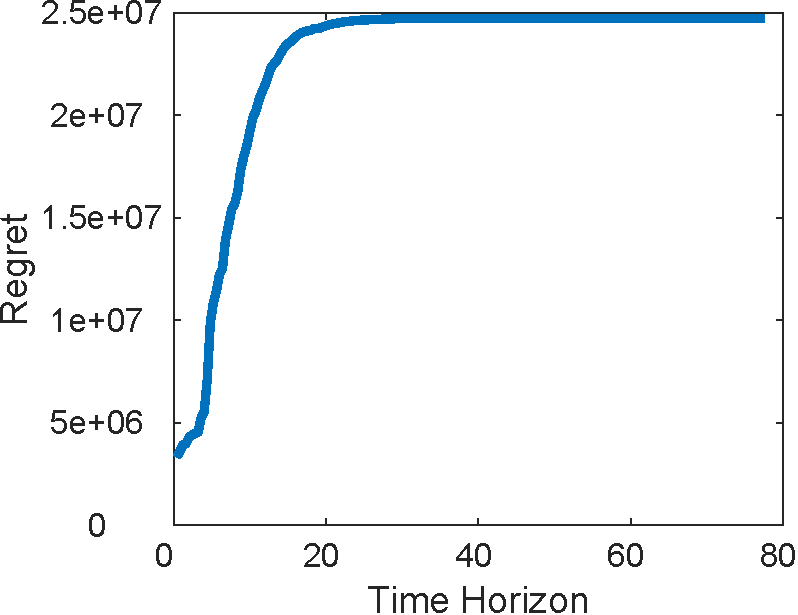
\includegraphics[width=.22\textwidth]{window1.pdf}
    \label{fig:0preview}}
     \subfigure[Regret vs. Time Horizon with $W=1$]{
         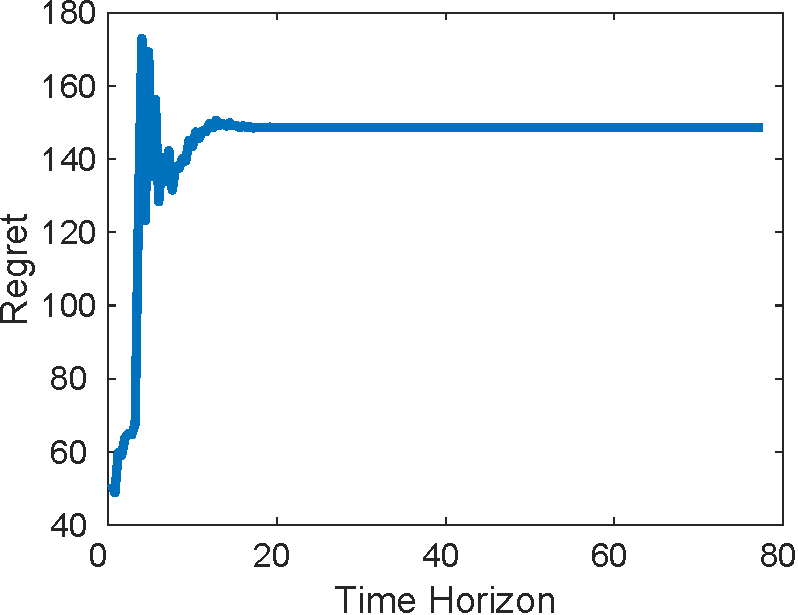
\includegraphics[width=.22\textwidth]{window2.pdf}
    \label{fig:1preview}}
    \\
     \subfigure[Regret vs. Preview Window Length in $T=8$]{
         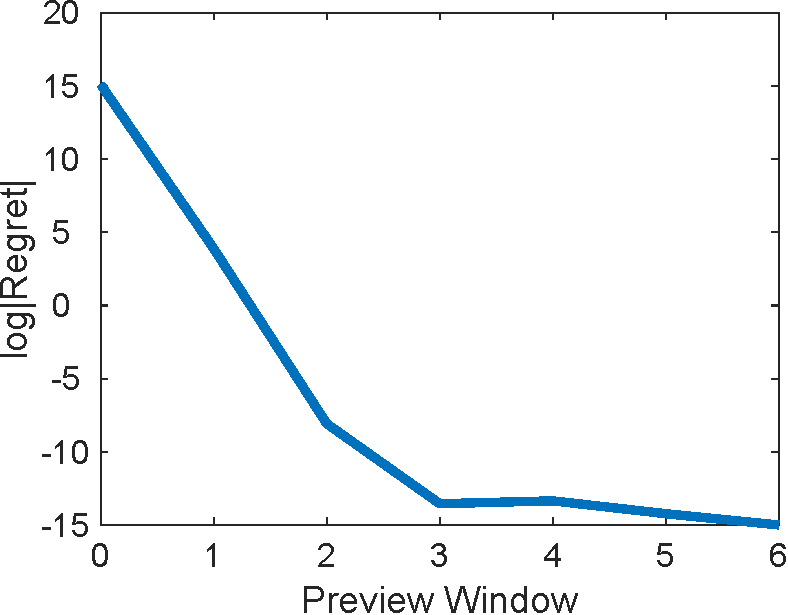
\includegraphics[width=.22\textwidth]{time1.pdf}
    \label{fig:8timehorizon}}
     \subfigure[Regret vs. Preview Window Length in $T = 70$]{
         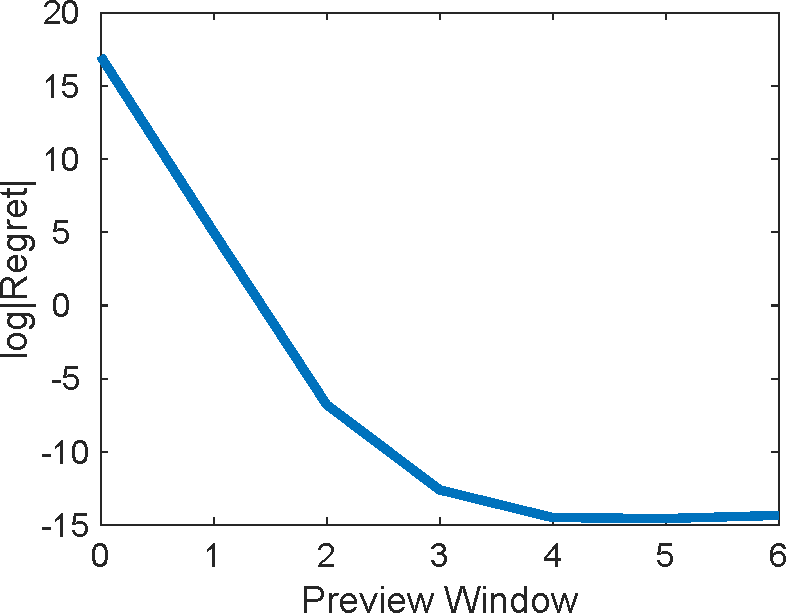
\includegraphics[width=.22\textwidth]{timeThird.pdf}
    \label{fig:69timehorizon}}
    \caption{Performance measure $\text{Regret}_{T}$ for simulated systems.}
\end{figure}

\section{CONCLUSIONS AND FUTURE WORKS}\label{sec:conclusions}
This paper proposes an online feedback potential game problem, a novel algorithm for this problem, and the analysis of its performance by \emph{dynamic social regret}, which is a natural extension of dynamic \emph{Regret} from \cite[Equation (5)]{chen_regret_2023} suggests that the algorithm yields a sublinear \emph{dynamic social regret}. This paper leads to many interesting research directions which are briefly discussed below. One can investigate the case of $N$-player potential dynamic game with time-varying $A_{t}$ and $\mathbf{B}_{t}$ for the system matrices. Another direction could be the case of a zero-sum LQ game when cost matrices are revealed sequentially to each player.


%%%%%%%%%%%%%%%%%%%%%%%%%%%%%%%%%%%%%%%%%%%%%%%%%%%%%%%%%%%%%%%%%%%%%%%%%%%%%%%%
% \section{ACKNOWLEDGMENTS}

% The authors gratefully acknowledge the contribution of National Research Organization and reviewers' comments.


%%%%%%%%%%%%%%%%%%%%%%%%%%%%%%%%%%%%%%%%%%%%%%%%%%%%%%%%%%%%%%%%%%%%%%%%%%%%%%%%

\bibliographystyle{plain}
\bibliography{References}
\appendix
% \section{Proof of Theorem~\ref{thm:main}}
Before stating the proof of Theorem~\ref{thm:main}, in the next subsection, we introduce the necessary lemmas and propositions. 
\subsection{Auxiliary Lemmas}
\begin{lemma}
    Define
        \begin{equation}\label{eq:Theta}
        [\Theta_{t}]_{ij} := [R_{t}]^{i}_{ij} + B^{i\transpose}P_{t+1}^{i}B^{j},t\in \mathbb{N}_{T},t\in\mathbb{N}_{T-1}
        \end{equation}
    where $R_{t}^{1},R_{t}^{2},Q_{t}$ satisfy Assumption \ref{assumption:bounds}, and
    \begin{equation*}
        P_{T}^{1} = P_{T}^{2}=Q_{T},
    \end{equation*}
        \begin{equation}\label{eq:costFPDG1}
            [R_{t}^{1}]_{12} + B^{1\transpose}P_{t+1}^{1}B^{2} = ([R_{t}^{2}]_{21} + B^{2\transpose}P_{t+1}^{2}B^{1})^{\transpose},
        \end{equation}
        \begin{equation}\label{eq:costFPDG2}
            \Theta_{t} \in \mathbb{S}_{++}^{2m},
        \end{equation}
        \begin{equation}\label{eq:costFPDG3}
            \mathbf{B}^{\transpose}(P_{t}^{1}-P_{t}^{2})A=0.
        \end{equation}
    Then, the LQDFG in the sense of Definition \ref{def:LQDFG} parameters is an LQDFPG in the sense of Definition \ref{def:LQDFPG}.
\end{lemma}
The above lemma is a special case of \cite[Theorem 6]{prasad_structure_2023} when $Q_{t}^{1}=Q_{t}^{2}$ for $t\in \mathbb{N}_T$.

\begin{lemma}[Theorem 5, \cite{prasad_structure_2023}]\label{lemma:gamePGrelation}
    Consider an LQDFPG and an LQOCP described by Definitions \ref{def:LQDFG} and \ref{def:LQOCP}, respectively. Under Assumption \ref{assumption:bounds}, the Feedback Nash Equlibrium for the LQDFPG defined in Definition \ref{def:LQDFG} by parameters $\{\bar{x}_{1},\{Q_{t}\}_{t=1}^{T},\{R_{t}^{i}\}_{i=1,t=1}^{2,T-1}\}$, is identical to the solutions of LQOCP defined in Definition \ref{def:LQOCP}, by parameters $\{\bar{x}_{1},\{\bar{Q}_{t}\}_{t=1}^{T},\{\bar{R}_{t}\}_{t=1}^{T-1}\}$, if
    \begin{align*}
        &\bar{P}_{T} = \bar{Q}_{T},\\
        &\bar{\Theta}_{t} = \bar{R}_{t} + \contB^{\transpose}\bar{P}_{t+1}\contB,\\
        &\bar{K}_{t} = \bar{\Theta}_{t}^{-1}\contB^{\transpose}\bar{P}_{t+1}A,\\
        &\bar{P}_{t} = \bar{Q}_{t} + \bar{K}_{t}^{\transpose}\bar{R}_{t}\bar{K}_{t} + (A+\contB\bar{K}_{t})^{\transpose}\bar{P}_{t+1}(A+\contB\bar{K}_{t}),\\
        &\bar{\Theta}_{t} \in \mathbb{S}_{++}^{2m},\\
        &[R_{t}^{i}]_{ii} + B^{i\transpose}P_{t+1}^{i}B^{i} = [\bar{R}_{t}]_{ii} + B^{i\transpose}\bar{P}_{t+1}B^{i},\\
        &B^{i\transpose}P_{t+1}^{i}A = B^{i\transpose}\bar{P}_{t+1}A,\\
        &[R_{t}^{i}]_{ij} + B^{i\transpose}P_{t+1}^{i}B^{j} = [\bar{R}_{t}]_{ij} + B^{i\transpose}\bar{P}_{t+1}B^{j},i\neq j,\\
        &[R_{t}^{1}]_{12} + B^{1\transpose}P_{t+1}^{1}B^{2} = ([R^{2}_{t}]_{21} + B^{2\transpose}P^{2}_{t+1}B^{1})^{\transpose},
    \end{align*}
    for $i,j\in \{1,2\}$ and $t \in \mathbb{N}_{T-1}$. 
\end{lemma}


\begin{lemma}[Theorem 7, \cite{prasad_structure_2023}]
    For a given positive integer $T$, define
        $\Omega := ((\bar{Q}_{1},\bar{Q}_{2},\cdots,\bar{Q}_{T},\bar{R}_{1},\cdots,\bar{R}_{T-1})|\mathcal{K})$,
    where $\mathcal{K}$ is the set of conditions that, at time instant $T$, $\bar{Q}_{T}$ is such that
            $\mathbf{B}^{\transpose}\bar{Q}_{T}A = \mathbf{B}^{\transpose}Q_{T}A$.
        Let $\bar{P}_{T}$ satisfy
            $\mathbf{B}^{\transpose}\bar{P}_{T}A = \mathbf{B}^{\transpose}Q_{T}A$, and define $\bar{R}_{t}$ as
            \begin{equation}\label{eq:matrixR}
            \bar{R}_{t} := \Theta_{t} - \mathbf{B}^{\transpose}\bar{P}_{t+1}\mathbf{B},
            \end{equation}
        where $\Theta_{t} \in \mathbb{S}_{++}^{2m}$,
        with $\bar{Q}_{t}$ such that
            $\bar{Q}_{t} = Q_{t} + K_{t}^{\transpose}(R_{t}^{1}-\bar{R}_{t})K_{t}$,
        where
        \begin{equation*}
            K_{t} = \Theta_{t}^{-1}
            \begin{bmatrix}
                B_{t}^{1\transpose}P_{t+1}^{1}\\
                B_{t}^{2\transpose}P_{t+1}^{2}
            \end{bmatrix}
            A,\quad t\in \mathbb{N}_{T-1}.
        \end{equation*}
    Every element in $\Omega$ leads to an LQOCP which is equivalent to an LQDFPG. Further, $\Omega$ is non-empty.
\end{lemma}

\begin{corollary}\label{corollary:boundedR}
    % There exists matrices $\bar{R}_{min},\bar{R}_{max} \in \mathbf{S}_{++}^{m}$, that the cost matrix defined in \eqref{eq:matrixR} satisfy the following
    Under Assumptions \ref{assumption:bounds} and \ref{assumption:controllable}, $\bar{R}_{t}$ defined in \eqref{eq:matrixR} satisfies $0 \prec R_{min} \preceq \bar{R}_{t} \preceq R_{max}$,
    for $t \in \mathbb{N}_{T-1}$.
\end{corollary}
\begin{proof}
    By definition of $\bar{R}_{t}$, we have
    \begin{align*}
        \bar{R}_{t} &= 
        \begin{bmatrix}
            [R_{t}^{1}]_{11} & [R_{t}^{1}]_{12}\\
            [R_{t}^{2}]_{21} & [R_{t}^{2}]_{22}
        \end{bmatrix}
        + 
        \begin{bmatrix}
            B^{1\transpose}P_{t+1}^{1}\\
            B^{2\transpose}P_{t+1}^{2}
        \end{bmatrix}\mathbf{B}
        - \mathbf{B}^{\transpose}\bar{P}_{t+1}\mathbf{B}\\
        &= \begin{bmatrix}
            [R_{t}^{1}]_{11} & [R_{t}^{1}]_{12}\\
            [R_{t}^{2}]_{21} & [R_{t}^{2}]_{22}
        \end{bmatrix}
        + 
        (\begin{bmatrix}
            B^{1\transpose}P_{t+1}^{1}\\
            B^{2\transpose}P_{t+1}^{2}
        \end{bmatrix}-
        \begin{bmatrix}
            B^{1\transpose}\bar{P}_{t+1}\\
            B^{2\transpose}\bar{P}_{t+1}
        \end{bmatrix}
        )\mathbf{B}
    \end{align*}
    Due to Assumption \ref{assumption:controllable}, $A$ is full-rank. Therefore, for $i \in \{1,2\}$,
        $B^{i\transpose}P_{t+1}^{i} = B^{i\transpose}\bar{P}_{t+1}$.
    Thus,
        $\bar{R}_{t} = 
        \begin{bmatrix}
            [R_{t}^{1}]_{11} & [R_{t}^{1}]_{12}\\
            [R_{t}^{2}]_{21} & [R_{t}^{2}]_{22}
        \end{bmatrix}$.
    The proof is complete in light of \eqref{eq:positiveR} (Assumption \ref{assumption:bounds}).
    % Suppose $x\in \mathbb{R}^{2m}$ is non-zero. Let $x = [x_{1:m} | x_{m+1:2m}]$, we have
    % \begin{align*}
    %     &x^{\transpose}\begin{bmatrix}
    %         [R_{t}^{1}]_{11} & [R_{t}^{1}]_{12}\\
    %         [R_{t}^{2}]_{21} & [R_{t}^{2}]_{22}
    %     \end{bmatrix}x \\
    %     &= x_{1:m}^{\transpose}[R_{t}^{1}]_{11}x_{1:m} + x_{m+1:2m}^{\transpose}[R_{t}^{2}]_{22}x_{m+1:2m} + x_{1:m}^{\transpose}[R_{t}^{1}]_{12}x_{m+1:2m} + x_{m+1:2m}^{\transpose}[R_{t}^{2}]_{21}x_{1:m}
    % \end{align*}
    % By using the properties of eigenvalues, we have
    % \begin{align*}
    %     \lambda_{min}([R_{t}^{1}]_{11}) + \lambda_{min}([R_{t}^{2}]_{22}) \leq x_{1:m}^{\transpose}[R_{t}^{1}]_{11}x_{1:m} + x_{m+1:2m}^{\transpose}[R_{t}^{2}]_{22}x_{m+1:2m} \leq \lambda_{max}([R_{t}^{1}]_{11}) + \lambda_{max}([R_{t}^{2}]_{22}).
    % \end{align*}
    % Moreover, define $y = U_{[R_{t}^{1}]_{12}}x_{1:m}$ and $z = V_{[R_{t}^{1}]_{12}}^{*}x_{m+1:2m}$,
    % \begin{align*}
    %     x_{1:m}^{\transpose}[R_{t}^{1}]_{12}x_{m+1:2m} &= \sum_{i=1}^{m} \lambda_{i}([R_{t}^{1}]_{12}x_{m+1:2m}) y_{i}z_{i} \\
    %     &\geq 0\\
    %     &\leq \lambda_{max}([R_{t}^{1}]_{12}).
    % \end{align*}
    % Similar procedures can be applied to matrix $[R_{t}^{2}]_{21}$. Therefore, 
    % \begin{align*}
    %     x^{\transpose}\begin{bmatrix}
    %         [R_{t}^{1}]_{11} & [R_{t}^{1}]_{12}\\
    %         [R_{t}^{2}]_{21} & [R_{t}^{2}]_{22}
    %     \end{bmatrix}x
    % \end{align*}
    % has finite eigenvalues. We can thus construct such $\bar{R}_{min}$ and $\bar{R}_{max}$ that
    % \begin{align*}
    %     0 \prec \bar{R}_{min} \preceq \bar{R}_{t} \preceq \bar{R}_{max},
    % \end{align*}
    % by eigen-decomposition of $\bar{R}_{t}$.
\end{proof}

\begin{remark}
    Based on the proof above, for any given $\tau$ and $t$, such that $1\leq \tau \leq t \leq T-1$, 
        $\bar{R}_{\tau|t} = \bar{R}_{\tau}$.
\end{remark}

\begin{lemma}\label{lemma:matrixK}
    Suppose $m \leq n$ and $R\in \mathbb{S}^{m}_{++}$. 
    If $P\in \mathbb{S}^{n}_{++}$, then for any given $B$ that has appropriate size and finite singular values, all singular values of matrix $K = (R+B^{\transpose}PB)^{-1}B^{\transpose}P$ satisfy the inequality
$  0 \leq \sigma_{k}(K) < \theta_{k}$,
    where $\sigma_{k}(\cdot)$ is the $k$-th singular value of its argument such that $\sigma_{1}(\cdot) \geq \cdots \geq \sigma_{m}(\cdot)$, and $\sigma_{\min}(B) < \theta_{k} <\sigma_{\max}(B)$.
\end{lemma}
\begin{proof}
    Due to matrix $K^{\transpose}K$ being symmetric and all elements are real, all eigenvalues of $K^{\transpose}K$ are real.
    Define an $n\times n$ matrix
        $\underbar{B} := 
        \begin{bmatrix}
            B & 0_{n\times n-m}
        \end{bmatrix}$,
    and suppose
    \begin{equation*}
        \lambda_{1}(B^{\transpose}K^{\transpose}KB) \geq \cdots \geq \lambda_{m}(B^{\transpose}K^{\transpose}KB).
    \end{equation*}
    Note that $       0 =  \lambda_{m+1}(B^{\transpose}K^{\transpose}KB) = \cdots = \lambda_{n}(B^{\transpose}K^{\transpose}KB)$,
    due to $\textit{rank}(B^{\transpose}K^{\transpose}KB) \leq m$.
    By using \cite[Theorem 4.5.9]{horn_matrix_2013} (see also the discussion on \cite[p.~284]{horn_matrix_2013}), for any $k$ such that $1\leq k\leq m\leq n$,  where $\textit{dim}(B)=m$,
    we have that
    \begin{align*}
        \lambda_{k}(B^{\transpose}K^{\transpose}KB) &= \lambda_{k}(\underbar{B}^{\transpose}K^{\transpose}K\underbar{B})= \theta_{k}\lambda_{k}(K^{\transpose}K),
    \end{align*}
    where $0\leq \theta_{k} \leq \sigma_{max}(\underbar{B})=\sigma_{max}(B)$.
    Due to
    \begin{align*}
        \sigma_{k}(KB) &= \sigma_{k}((R+B^{\transpose}PB)^{-1}B^{\transpose}PB)\\
        &= \sigma_{k}\bigg((I - (R+B^{\transpose}PB)^{-1}R) \bigg),
    \end{align*}
    and
       $0 \leq \sigma_{k}\bigg((I - (R+B^{\transpose}PB)^{-1}R) \bigg) < 1$,
    when $P \in \mathbb{S}_{++}^{n}$. This is due to the following. Consider a scalar $\sigma$ and matrix
    \begin{align*}
        &G := (I-(\tempRBP)^{-1}R)^{\transpose}(I-(\tempRBP)^{-1}R) - (1-\sigma) I \\
        &= \sigma I - R(\tempRBP)^{-1} \\
        &\quad - (\tempRBP)^{-1}R + R(\tempRBP)^{-1}(\tempRBP)^{-1}R\\
        &= R\bigg(\sigma R^{-2}- (\tempRBP)^{-1}R^{-1} - R^{-1}(\tempRBP)^{-1}\\
        &\quad + (\tempRBP)^{-1}(\tempRBP)^{-1} \bigg)R\\
        &= R(\tempRBP)^{-1}\bigg(\sigma(\tempRBP)R^{-1}R^{-1}(\tempRBP) \\
        &\quad - R^{-1}(\tempRBP) - (\tempRBP)R^{-1} + I \bigg)(\tempRBP)^{-1}R\\
        &= R(\tempRBP)^{-1}\bigg(\sigma(I+B^{\transpose}PBR^{-1})(I+R^{-1}B^{\transpose}PB)\\
        &\quad  - R^{-1}(\tempRBP) - (\tempRBP)R^{-1} + I \bigg)(\tempRBP)^{-1}R\\
        &= R(\tempRBP)^{-1}\bigg((\sigma-1)(I+B^{\transpose}PBR^{-1}+R^{-1}B^{\transpose}PB)\\
        &\quad  + \sigma(B^{\transpose}PBR^{-1}R^{-1}B^{\transpose}PB)\bigg)(\tempRBP)^{-1}R.
    \end{align*}
    Therefore, if $\det(G) = 0$, then there exist zero eigenvalue of $(\sigma-1)(I+B^{\transpose}PBR^{-1}+R^{-1}B^{\transpose}PB) + \sigma(B^{\transpose}PBR^{-1}R^{-1}B^{\transpose}PB)$.

    Since $B^{\transpose}PBR^{-1}R^{-1}B^{\transpose}PB = (R^{-1}B^{\transpose}PB)^{\transpose}(R^{-1}B^{\transpose}PB)(:= G^{'})$, therefore
        $\lambda_{k}(B^{\transpose}PBR^{-1}R^{-1}B^{\transpose}PB) \geq 0$, $k\in  \mathbb{N}_m$.
    Moreover, Let $\bar{G} := I+B^{\transpose}PBR^{-1}+R^{-1}B^{\transpose}PB$, 
    Suppose $\lambda_{1}(\bar{G}) \geq \cdots \geq \lambda_{m}(\bar{G})$. By Weyl's inequality, for $ k \in \mathbb{N}_m$, we have
    \begin{equation}\label{eq:eigenStep3}
        \lambda_{k}(I) + \lambda_{m}(B^{\transpose}PBR^{-1}+R^{-1}B^{\transpose}PB) \leq \lambda_{k}(\bar{G}).
    \end{equation}
    
    By applying Weyl's inequality again, and due to 
    \begin{align*}
        B^{\transpose}PBR^{-1} = R^{\frac{1}{2}}(R^{-\frac{1}{2}}B^{\transpose}PBR^{-\frac{1}{2}})R^{\frac{1}{2}},
    \end{align*}
    we have all eigenvalues of $B^{\transpose}PBR^{-1}$ are greater than 0. Similarly to $R^{-1}B^{\transpose}PB$.
    Therefore,
    \begin{equation}\label{eq:eigenStep4}
        0 < 1 \leq \lambda_{k}(I) + \lambda_{m}(B^{\transpose}PBR^{-1})+\lambda_{m}(R^{-1}B^{\transpose}PB) \leq \lambda_{k}(\bar{G}).
    \end{equation}

     We can further conclude that
     \begin{align*}
         (\sigma-1)\lambda_{k}(G^{'})+\sigma\lambda_{m}(\bar{G}) \leq \lambda_{k}(G) \leq (\sigma-1)\lambda_{k}(G^{'})+\sigma\lambda_{1}(\bar{G}).
     \end{align*}
     If $\sigma \geq 1$, due to
     \begin{align*}
         (\sigma-1)\lambda_{k}(G^{'})+\sigma\lambda_{m}(\bar{G}) \leq \lambda_{k}(G) \leq (\sigma-1)\lambda_{k}(G^{'})+\sigma\lambda_{1}(\bar{G}),
     \end{align*}
     we have $(\sigma-1)\lambda_{k}(G^{'})+\sigma\lambda_{m}(\bar{G}) > 0$,
     therefore $\lambda_{k}(G) > 0(k \in \mathbb{N}_{n})$. If $\sigma < 0$, $(\sigma-1)\lambda_{k}(G^{'})+\sigma\lambda_{m}(\bar{G}) < 0$ and $\lambda_{k}(G) \leq (\sigma-1)\lambda_{k}(G^{'})+\sigma\lambda_{1}(\bar{G}) < 0$.
     
     Therefore $\lambda_{k}(G) < 0$, $k \in \mathbb{N}_{n})$. Thus, $0 \leq \sigma < 1$.
    Consequently, all singular values of matrix $I - (R+B^{\transpose}PB)^{-1}R$ are between 0 and 1. Hence,
        $0 \leq \sigma_{k}(K) < \theta_{k}$, for $k \in \mathbb{N}_{n}$.
\end{proof}

\begin{corollary}\label{corrolary:boundedK}
    Suppose the cost matrices $(Q_{t})_{t=1}^{T}$ and $(R_{t}^{i})_{t=1,i=1}^{T-1,2}$ satisfy the conditions described from Equation \eqref{eq:costFPDG1} to \eqref{eq:costFPDG3} and Assumption \ref{assumption:bounds}.
    For a given preview horizon $W\in \mathbb{N}_{T-1}$, define
    \begin{equation}
        Q_{\tau|t}:= 
        \begin{cases}
            Q_{\tau} \text{ if $1\leq \tau \leq t+W$}\\
            Q_{t+W} \text{ if $t+W < \tau \leq T$},
        \end{cases}
    \end{equation}
    and
    \begin{equation}
        R_{\tau|t}^{i}:= 
        \begin{cases}
            R_{\tau}^{i} \text{ if $1\leq \tau \leq t+W$}\\
            R_{t+W}^{i} \text{ if $t+W < \tau \leq T$},
        \end{cases}
    \end{equation}
    for $i = {1,2}$.
    There exists a scalar $\omega_{K}$ such that
        $\|K_{\tau|t}\| \leq \omega_{K}$,
    for $1\leq \tau,t\leq T$.
\end{corollary}

\begin{proof}
    This can be directly concluded by letting $\omega_{K} = \sigma_{max}(B)\sigma_{max}(A)$ and applying Lemma \ref{lemma:matrixK}.
\end{proof}

\begin{corollary}
    For any given $\tau,t\in\mathbb{N}_{T-1}$, 
       $ \bar{Q}_{\tau|t} = Q_{\tau|t} + K_{\tau|t}^{\transpose}(R_{\tau|t}^{1} - \bar{R}_{\tau|t})K_{\tau|t} \in \mathbb{S}^{n}_{++}$.
\end{corollary}
\begin{proof}
    Suppose
    \begin{align*}
        &\lambda_{1}(Q_{\tau|t}) \geq \cdots \geq \lambda_{n}(Q_{\tau|t}),\\
        &\lambda_{1}(K_{\tau|t}^{\transpose}(R_{\tau|t}^{1} - \bar{R}_{\tau|t})K_{\tau|t}) \geq \cdots \geq \lambda_{n}(K_{\tau|t}^{\transpose}(R_{\tau|t}^{1} - \bar{R}_{\tau|t})K_{\tau|t}),\\
        &\lambda_{1}(R_{\tau|t}^{1} - \bar{R}_{\tau|t}) \geq \cdots \geq \lambda_{n}(R_{\tau|t}^{1} - \bar{R}_{\tau|t}).
    \end{align*}
    By Weyl's inequality,
    \begin{align*}
        \lambda_{min}(\bar{Q}_{\tau|t}) = \lambda_{n}(\bar{Q}_{\tau|t})\geq \lambda_{n}(Q_{\tau|t}) + \lambda_{n}(K_{\tau|t}^{\transpose}(R_{\tau|t}^{1} - \bar{R}_{\tau|t})K_{\tau|t}).
    \end{align*}
    By \cite[Theorem 4.5.9]{horn_matrix_2013}, there exists a positive scalar $\theta_{n}$ such that
        $\lambda_{n}(K_{\tau|t}^{\transpose}(R_{\tau|t}^{1} - \bar{R}_{\tau|t})K_{\tau|t}) = \theta_{n}\lambda_{min}(R_{\tau|t}^{1} - \bar{R}_{\tau|t})$,
    where $\sigma_{min}(K_{\tau|t}) \leq \theta_{n} \leq \sigma_{max}(K_{\tau|t}) < \sigma_{max}(B)$.
    The last inequality is due to Lemma \ref{lemma:matrixK}. 
    Moreover,
    \begin{align*}
        \max(0, \sigma_{max}(\contB)\lambda_{max}(\bar{R}_{t}-R_{t}^{1})) > -\lambda_{min}(K_{\tau|t}^{\transpose}(R_{t}^{1}-\bar{R}_{t})K_{\tau|t}).
    \end{align*}
    Thus, by Assumption \ref{assumption:lowerQ} and Corollary \ref{corollary:boundedR}, we have
    \begin{align*}
    0 &<  \lambda_{min}(Q_{\tau|t}) -\max(0,\sigma_{max}(\contB)\lambda_{max}([R_{t}^{2}]_{22} - [R_{t}^{1}]_{22}))\\
    &=\lambda_{min}(Q_{\tau|t}) - \max(0, \sigma_{max}(\contB)\lambda_{max}(\bar{R}_{t}-R_{t}^{1})) \\
    &< \lambda_{min}(Q_{\tau|t}+K_{t}^{\transpose}(R_{\tau|t}^{1}-\bar{R}_{\tau|t})K_{\tau|t})= \lambda_{min}(\bar{Q}_{\tau|t}).
    \end{align*}
    % \lambda_{min}(\bar{Q}_{\tau|t}) &= \lambda_{min}(Q_{\tau|t}+K_{t}^{\transpose}(R_{\tau|t}^{1}-\bar{R}_{\tau|t})K_{\tau|t})
         % &>\lambda_{min}(Q_{\tau|t}) - \max(0,\sigma_{B}\lambda_{min}(R_{\tau|t}^{1} - \bar{R}_{\tau|t}))
    % Moreover,
    % \begin{align*}
    %     \theta_{n}\lambda_{min}(R_{\tau|t}^{1} - \bar{R}_{\tau|t}) \geq \max(0,\sigma_{B}\lambda_{min}(R_{\tau|t}^{1} - \bar{R}_{\tau|t})).
    % \end{align*}
    % Thus, 
    % \begin{align*}
    %     \lambda_{min}(\bar{Q}_{\tau|t}) &= \lambda_{min}(Q_{\tau|t}+K_{t}^{\transpose}(R_{\tau|t}^{1}-\bar{R}_{\tau|t})K_{\tau|t}) \\
    %     &> \lambda_{min}(Q_{\tau|t}) +\max(0,\sigma_{B}\lambda_{min}(R_{\tau|t}^{1} - \bar{R}_{\tau|t})) > 0.
    % \end{align*}
    Therefore, $\bar{Q}_{\tau|t}$ is positive definite for all $t,\tau \in \mathbb{N}_{T}$.
\end{proof}

\begin{remark}
    Assumption \ref{assumption:lowerQ} suggests that, if the distance between the cost matrices $R_{t}^{2}$ and $R_{t}^{1}$ is sufficiently small, or $R_{t}^{1}$ is a dominant cost than $R_{t}^{2}$, then matrix $Q_{\tau|t}$ are positive definite. This will help us to develop the contraction between $K_{\tau|t}$ and $K_{\tau|t_{0}}$ for $\tau \in \mathbb{N}_t$ and $t_{0} \in \mathbb{N}_{T-1}$.
\end{remark}
\begin{assumption}
    The LQDFG with parameters $\{Q_{\tau|t}\}_{\tau=1}^{T}$ and $\{R_{\tau|t}\}_{\tau=1}^{T-1}$ is an LQDFPG for all $t\in \mathbb{N}_{T}$.
\end{assumption}
\begin{lemma}\label{lemma:boundedP}
Let $\bar{P}_{T} = \bar{Q}_{T}$ and 
    \begin{align*}
        \bar{K}_{t}& = -(R_{t}+ B^{\transpose}\bar{P}_{t+1}B)^{-1}B^{\transpose}\bar{P}_{t+1},\\
        \bar{P}_{t}& = \bar{Q}_{t} + \bar{K}_{t}^{\transpose}\bar{R}_{t}\bar{K}_{t} + (A+B\bar{K}_{t})^{\transpose}\bar{P}_{t+1}(A+B\bar{K}_{t}),
    \end{align*}
    for $t \in \mathbb{N}_{T-1}$. There exist positive definite matrices $\bar{P}_{min}$ and $\bar{P}_{max}$ such that $
        \bar{P}_{min} \preceq \bar{P}_{t} \preceq \bar{P}_{max}$.
\end{lemma}
\begin{proof}
    By Corrollary \ref{corrolary:boundedK} and Assumption \ref{assumption:lowerQ}, there exist positive definite matrices $\bar{Q}_{min},\bar{Q}_{max}$ such that $
        \bar{Q}_{min} \preceq \bar{Q}_{t} \preceq \bar{Q}_{max}$,
    for $t\in\mathbb{N}_{T}$.
    This, together with the Assumption \ref{assumption:bounds} and following a similar procedure to the proof of \cite[Proposition 11]{zhang_regret_2021} complete the proof.
\end{proof}


\begin{lemma}\label{lemma:m}
    For $T,S,V_{1},V_{2}\in \mathbb{S}_{++}^{n}$, if
$       m \geq 1+\frac{\lambda_{max}(V_{1}-V_{2})}{\lambda_{min}(T+V_{2})}$,
    then for any non-zero $x$, we have
    \begin{equation}
        \frac{\quadinner{T+V_{1}}}{\quadinner{S+V_{2}}} \leq m\frac{\quadinner{T+V_{2}}}{\quadinner{S+V_{2}}}
    \end{equation}
\end{lemma}
\begin{proof}
    For any nonzero $x$, we have
    \begin{align*}
        m \geq 1+\frac{\lambda_{max}(V_{1}-V_{2})}{\lambda_{min}(T+V_{2})}
        \geq 1+ \frac{\quadinner{V_{1}-V_{2}}}{\quadinner{T+V_{2}}}
        = \frac{\quadinner{T+V_{1}}}{\quadinner{T+V_{2}}}.
     \end{align*}
     Due to $\quadinner{S+V_{2}} > 0$ and the fact that $T,V_{2},V_{1}$ are positive definite, we have that 
         $m\frac{\quadinner{T+V_{2}}}{\quadinner{S+V_{2}}} \geq \frac{\quadinner{T+V_{1}}}{\quadinner{S+V_{2}}}$.
\end{proof}



% \begin{lemma}[Not sure again]
%     If the above lemma is true, we expect there exists $\bar{Q}_{min},\bar{Q}_{max}(\|\bar{Q}_{min}\|,\|\bar{Q}_{max}\|<\infty)$ that
%     \begin{equation*}
%         \bar{Q}_{min} \preceq \bar{Q}_{t} \preceq \bar{Q}_{max},
%     \end{equation*}
%     for $t\in\mathbb{N}_{T}$. Which
%     \begin{equation*}
%         \bar{Q}_{t} = Q_{t}+ \mathbf{K}_{t}^{\transpose}(R_{t}^{1}-\bar{R}_{t})\mathbf{K}_{t},
%     \end{equation*}
%     $\Theta_{t}$ is defined by \eqref{eq:Theta}
%     and $\mathbf{K}_{t}$ is defined by
%     \begin{equation*}
%         \mathbf{K}_{t} = -(\Theta_{t}^{-1})
%         \begin{bmatrix}
%             B^{1\transpose}P_{t+1}^{1} \\
%             B^{2\transpose}P_{t+1}^{2}
%         \end{bmatrix}A.
%     \end{equation*}
%     Which
%     \begin{equation*}
%         P_{t}^{i} = Q_{t} + \mathbf{K}_{t}^{\transpose}R_{t}^{i}\mathbf{K}_{t} + (A+\mathbf{B}\mathbf{K}_{t})^{\transpose}P_{t+1}^{i}(A+\mathbf{B}\mathbf{K}_{t}),
%     \end{equation*}
%     for $i = (1,2)$, $t \in \mathbb{N}_{T-1}$, and
%     \begin{equation*}
%         P_{T}^{i} = Q_{T},
%     \end{equation*}
%     for $i = (1,2)$,
%     recursively.
% \end{lemma}

\begin{definition}
    For any $X,Y\in \mathbb{S}_{++}^{n}$, define the operator $\delta_{\infty}(\cdot, \cdot)$ as
  $ \delta_{\infty}(X, Y) := \| \log(Y^{-\frac{1}{2}}XY^{-\frac{1}{2}})\|_{\infty}$, where $\|\cdot\|_{\infty}$ denotes the matrix infinity-norm.
        % \delta_{\infty}(X, Y) := (\sum_{i=1}^{d} \log^{2}(\lambda_{i}))^{\frac{1}{2}},
    % where $\lambda_{1},\cdots, \lambda_{d}$ are the eigenvalues of the matrix $XY^{-1}$.
\end{definition}

\begin{proposition}\label{proposition:deltaRatio}
    For any $X,Y\in \mathbb{S}_{++}^{n}$,
$ \delta_{\infty}(X,Y) = \max(\log(\sup_{\xi\neq0} \frac{\xi^{\transpose}X\xi}{\xi^{\transpose}Y\xi},\log(\sup_{\xi\neq0} \frac{\xi^{\transpose}Y\xi}{\xi^{\transpose}X\xi})$).
\end{proposition}
\begin{proof}
    Suppose matrices $X,Y\in\mathbb{S}_{++}^{n}$. From \cite[Remark 2.2.]{lee_invariant_2008}, $\delta_{\infty}(X,Y) = \max(\lambda_{max}(Y^{-1}X),\lambda_{max}(XY^{-1})), = \max(\log(\sup_{\xi\neq0} \frac{\xi^{\transpose}X\xi}{\xi^{\transpose}Y\xi}),\log(\sup_{\xi\neq0} \frac{\xi^{\transpose}Y\xi}{\xi^{\transpose}X\xi}))$.
\end{proof}

\begin{remark}\label{remark:delta}
    For $T,S,V_{1},V_{2}\in \mathbb{S}_{++}^{n}$, without loss of generality, assume
    $\sup_{x\neq 0} \frac{\quadinner{T+V_{1}}}{\quadinner{S+V_{2}}} \geq 1$.
    Based on Lemma \ref{lemma:boundedP},\ref{lemma:m} and Proposition \ref{proposition:deltaRatio}, suppose a positive scalar $m$ satisfies
    \begin{align*}
        m \geq 1+\frac{\lambda_{max}(V_{1}-V_{2})}{\lambda_{min}(T+V_{2})}.
    \end{align*}
   Consequently, 
    \begin{align*}
        \delta_{\infty}(T+V_{1},S+V_{2}) &= \log( \sup_{x\neq 0} \frac{\quadinner{T+V_{1}}}{\quadinner{S+V_{2}}})\\
        &\leq \log(\sup_{x\neq 0} \frac{\quadinner{T+V_{1}}}{\quadinner{S+V_{2}}})\\
        &\leq \log(m)+\log(\sup_{x\neq 0} \frac{\quadinner{T+V_{2}}}{\quadinner{S+V_{2}}})\\
        &\leq \log(m) + \delta_{\infty}(T+V_{2},S+V_{2})\\
        &\leq \log(m) + \gamma\delta_{\infty}(T,S),
    \end{align*}
    where $\gamma$, $0<\gamma<1$, can be found by \cite[Lemma D.2]{krauth_finite-time_2019}.
\end{remark}

\begin{lemma}\label{lemma:boundedPK}
    Suppose the preview window length is given by a non-negative integer $W\in \mathbb{N}_{T-1}$. For any $\tau$, $t$, and $t_{0}$ such that $1\leq \tau\leq t\leq t_{0}\leq T$, there exist positive scalars $\gamma,\varepsilon_{P},\varepsilon_{K},C_{P},C_{K}^{'}$ with $\gamma \in (0,1)$, such that
    \begin{equation*}
        \|\bar{P}_{\tau|t}-\bar{P}_{\tau|t_{0}}\| \leq C_{P}\gamma^{t-\tau+W}+\varepsilon_{P},
    \end{equation*}
    and
        $\|\bar{K}_{\tau|t}-\bar{K}_{\tau|t_{0}}\| \leq C_{K}^{'}\gamma^{t-\tau+1+W}+\varepsilon_{K}^{'}$.
\end{lemma}
\begin{proof}
     For any $\tau$ ,$t$, $t_{0}$ where $1\leq \tau\leq t\leq t_{0}\leq T$, 
     let
     \begin{align*}
        &\alpha_{\tau,t} := \lambda_{max}(A^{\transpose}(\bar{P}_{\tau+1|t}^{-1}+B\bar{R}_{\tau|t}^{-1}B^{\transpose})^{-1}A)\\
        &\beta_{\tau,t} := \lambda_{min}(\bar{Q}_{\tau|t})\\ 
        &\gamma := \max_{1\leq \tau,t \leq T} \frac{\alpha_{\tau,t}}{\alpha_{\tau,t}+\beta_{\tau,t}}. 
     \end{align*}
     By \cite[Lemma D.2]{krauth_finite-time_2019}, Lemmas \ref{lemma:boundedP} and \ref{lemma:m}, and Remark \ref{remark:delta}, we have 
    \begin{align*}
        \delta_{\infty}(\bar{P}_{\tau|t},\bar{P}_{\tau|t_{0}}) &= \delta_{\infty}(\bar{Q}_{\tau|t}+A^{\transpose}(\bar{P}_{\tau+1|t}^{-1}+B\bar{R}_{\tau|t}^{-1}B^{\transpose})^{-1}A,\\
        & \qquad \bar{Q}_{\tau|t_{0}}+A^{\transpose}(\bar{P}_{\tau+1|t_{0}}^{-1}+B\bar{R}_{\tau|t_{0}}^{-1}B^{\transpose})^{-1}A)\\
        % &\leq \delta_{\infty}(Q_{\tau}+K_{\tau|t}^{\transpose}(R_{\tau}^{1}-\bar{R}_{\tau})K_{\tau|t}+A^{\transpose}(P_{\tau+1|t}^{-1}+B\bar{R}_{\tau|t}^{-1}B^{\transpose})^{-1}A,\\
        % & \qquad Q_{\tau}+K_{\tau|t_{0}}^{\transpose}(R_{\tau}^{1}-\bar{R}_{\tau})K_{\tau|t_{0}}+A^{\transpose}(P_{\tau+1|t_{0}}^{-1}+B\bar{R}_{\tau|t_{0}}^{-1}B^{\transpose})^{-1}A)\\
        &\leq \gamma\delta_{\infty}(\bar{P}_{\tau+1|t},\bar{P}_{\tau+1|t_{0}}) + \varepsilon_{1}\\
        &\leq \gamma^{t-\tau+W}\delta_{\infty}(\bar{P}_{t+W|t},\bar{P}_{t+W|t_{0}}) + \varepsilon_{1}\sum_{p=0}^{t-\tau+W}\gamma^{p}\\
        % &< \gamma^{t-\tau+W}\delta_{\infty}(\bar{P}_{t+W|t},\bar{P}_{t+W|t_{0}}) + \frac{\varepsilon_{1}}{1-\gamma}\\
        &\leq C_{P_{1}}\gamma^{t-\tau+W}+\frac{\varepsilon_{1}}{1-\gamma},
    \end{align*}
    where $\varepsilon_{1}$ can be found as similar as the term $\log(m)$ from Remark \ref{remark:delta}, and $C_{P1} = \max_{t\leq t_{0}} \delta_{\infty}(\bar{P}_{t|t},\bar{P}_{t|t_{0}})$ . 
    % By inequality
    %\begin{align*}
    %    \frac{e^{x}-1}{x} \leq \frac{e^{c}-1}{c},
    %\end{align*}
    %for $0 < x \leq c$. 
Let $h = \max_{(\tau,t_{0}| \tau,\leq t_{0})} \delta_{\infty}(\bar{P}_{\tau|t},\bar{P}_{\tau|t_{0}})$, we have
    \begin{equation*}
        \frac{exp(\delta_{\infty}(\bar{P}_{\tau|t},\bar{P}_{\tau|t_{0}}))-1}{\delta_{\infty}(\bar{P}_{\tau|t},\bar{P}_{\tau|t_{0}})} \leq \frac{exp(h)-1}{h}.
    \end{equation*}
    Thus,
    \begin{align*}
        \|\bar{P}_{\tau|t}-\bar{P}_{\tau|t_{0}}\| &\leq \lambda_{max}(\bar{P}_{\tau|t_{0}})\frac{\exp(h)-1}{h}\delta_{\infty}(\bar{P}_{\tau|t},\bar{P}_{\tau|t_{0}})\\
        &< C_{P}\gamma^{W}+\varepsilon_{P},
    \end{align*}
    where $C_{P} = \frac{C_{P1}\lambda_{max}(\bar{P}_{\tau|t_{0}})(\exp(h)-1)}{h}$ and $\varepsilon_{P} = \frac{\varepsilon_{1}\lambda_{max}(\bar{P}_{\tau|t_{0}})(\exp(h)-1)}{h(1-\gamma)}$. Following by similar steps of equations (20) and (21) from \cite[Lemma 8]{chen_regret_2023}, we can find $C_{K}^{'},\varepsilon_{K}^{'}(C_{K}^{'}>0,\varepsilon_{K}^{'}>0)$ we have that $\|\bar{K}_{\tau|t}-\bar{K}_{\tau|t_{0}}\| \leq C_{K}^{'}\gamma^{t-\tau-1+W}+\varepsilon_{K}^{'}$.
    % \begin{align*}
    %     \|\bar{K}_{\tau|t}-\bar{K}_{\tau|t_{0}}\| \leq C_{K}^{'}\gamma^{t-\tau-1+W}+\varepsilon_{K}^{'}.
    % \end{align*}
\end{proof}

\begin{remark}
    When $\tau = t$ and $t_{0} = T$, we have
    \begin{align*}
        \|\bar{K}_{t|t}-\bar{K}_{t}^{*}\| \leq C_{K}^{'}\gamma^{W-1} + \varepsilon_{K}^{'}.
    \end{align*}
\end{remark}

\begin{lemma}\label{lemma:multGain}
    For time horizon $T$, suppose $1\leq t_{0} \leq t_{1}\leq t\leq T-1$. There exist positive scalars such that
    \begin{equation*}
        \left \| \prod_{\tau=t_{0}}^{t_{1}}(A+\mathbf{B}\bar{K}_{\tau|t})  \right\| \leq C_{fb}\eta^{t_{1}-t_{0}+1},\text{ and }\eta<1.
    \end{equation*}
\end{lemma}
This lemma can be proved following the same steps as those found in the proof of \cite[Appendix E,Proposition 2]{zhang_regret_2021}.
\begin{lemma}
    Suppose the preview window horizon is given by a non-negative integer $W\in\mathbb{N}_{T-1}$, there exists a positive scalar $q\in(0,1)$, such that the distance between state $x_{t}$ and $x_{t|t}$ has an upperbound of
    \begin{equation*}
    \begin{split}
        \|x_{t}-x_{t|t}\| &\leq C_{fb}^{2}\|\bar{x}_{1}\|q^{t} \left [\frac{C_{K}\gamma^{W}}{\gamma-1}\bigg(\frac{1-(\frac{\eta\gamma}{q})^{t}}{1-\frac{\eta\gamma}{q}} - \frac{1-(\frac{\eta}{q})^{t}}{1-\frac{\eta}{q}} \bigg) \right .\\
        &\left . +\varepsilon_{K}\bigg(\frac{(t-1)(\frac{\eta}{q})^{t+1}-t(\frac{\eta}{q})^{t}+\frac{\eta}{q}}{(1-\frac{\eta}{q})^{2}}\bigg) \right ].  \end{split}
    \end{equation*}
\end{lemma}
\begin{proof}
    Suppose $N$ is a positive integer. For an arbitrary sequence $(a_{i})_{i=1}^{N}$. Suppose $e$ is the identity element for the sequence. For $1\leq p_{1},p_{2}\leq N$, define the product operator as
\begin{equation*}
    \prod_{j=p_{1}}^{p_{2}} a_{j} := 
    \begin{cases}
        a_{p_{2}}a_{p_{2}-1}\dots a_{p_{1}} & \text{if $p_{1} < p_{2}$}\\
        a_{p_{2}} & \text{if $p_{1} = p_{2}$}\\
        e & \text{if $p_{1} > p_{2}$},
    \end{cases}
\end{equation*}
Define $\omega_{t} := x_{t}-x_{t|t}$, $\theta_{\tau| p_{1},p_{2}} := x_{\tau|p_{1}}-x_{\tau|p_{2}}$, where $\tau \leq p_{1}\leq p_{2}\leq T$. Consequently, $w_{1} = 0$ and $\theta_{1|p_{1},p_{2}}=0$. We now investigate the dynamics of $w_{t}$ and $\theta_{\tau|p_{1},p_{2}}$. For integer $\tau > 1$:
\begin{align*}
    &\theta_{\tau|p_{1},p_{2}}= x_{\tau|p_{1}}-x_{\tau|p_{2}}\\
    &= (A+\sum_{j}^{2}B^{j}K_{j,\tau|p_{1}})x_{\tau-1|p_{1}} - (A+\sum_{j}^{2}B^{j}K_{j,\tau|p_{2}})x_{\tau-1|p_{2}}\\
    &= (A+\sum_{j}^{2}B^{j}K_{j,\tau|p_{1}})\theta_{\tau-1|p_{1},p_{2}} + [\sum_{j=1}^{2} B^{j}(K_{j,\tau-1|p_{1}}-K_{j,\tau-1|p_{2}})]x_{\tau-1|p_{2}}\\
    &\qquad \vdots\\
    &= \sum_{i=1}^{\tau-1}\bigg(\prod_{j=i+1}^{\tau-1}(A+\sum_{m=1}^{2}B^{m}K_{m,j|p_{1}})\bigg)\bigg[\sum_{m=1}^{2}B^{m}(K_{m,i|p_{1}}-K_{m,i|p_{2}})\bigg]x_{i|p_{2}}  \\
    &= \sum_{i=1}^{\tau-1}\bigg(\prod_{j=i+1}^{\tau-1}(A+\sum_{m=1}^{2}B^{m}K_{m,j|p_{1}})\bigg)\bigg[\sum_{m=1}^{2}B^{m}(K_{m,i|p_{1}}-K_{m,i|p_{2}})\bigg]\\
    &\qquad\bigg(\prod_{n=1}^{i-1} (A+\sum_{m=1}^{2}B^{m}K_{m|p_{2}})\bigg)\bar{x}_{1}\\
    &= \sum_{i=1}^{\tau-1}\bigg(\prod_{j=i+1}^{\tau-1}(A+\mathbf{B}\bar{K}_{j|p_{1}})\bigg)\bigg[\mathbf{B}^{\mathsf{T}}(\bar{K}_{j|p_{1}}^{\mathsf{T}}-\bar{K}_{j|p_{2}}^{\mathsf{T}})\bigg]\\
    &\qquad\bigg(\prod_{n=1}^{i-1}(A+\mathbf{B}\bar{K}_{n|p_{2}})\bigg)\bar{x}_{1}.
\end{align*}
Thus, for integer $t\in\mathbb{N}_T$, we have
\begin{align*}
    \omega_{t} &= x_{t} - x_{t|t}\\
    &= Ax_{t-1} + \sum_{j=1}^{2}B^{j}[K^{j}(x_{t-1}-x_{t-1|t-1})+K_{t-1|t-1}^{j}x_{t-1|t-1}] - x_{t|t}\\
    &= (A+\sum_{j=1}^{2}B^{j}K^{j})x_{t-1} + [\sum_{j=1}^{2}B^{j}(K_{t-1|t-1}^{j}-K^{j})]x_{t-1|t-1} - x_{t|t}\\
    &= (A+\sum_{j=1}^{2}B^{j}K^{j})(x_{t-1}-x_{t-1|t-1}) + x_{t|t-1}-x_{t|t}\\
    &= \sum_{i=1}^{t} (A+\sum_{j=1}^{2}B^{j}K^{j})^{t-i} \theta_{i|i-1,i}.
\end{align*}

We now investigate the dynamics of $\theta_{\tau|p_{1},p_{2}}$. Note that $\theta_{0|p_{1},p_{2}} = 0$, and 
\begin{align*}
    \theta_{\tau+1|p_{1},p_{2}} &= x_{\tau+1|p_{1}} - x_{\tau+1|p_{2}}\\
    &= (A+\BK{\tau|p_{1}})x_{\tau|p_{1}}-(A+\BK{\tau|p_{2}})x_{\tau|p_{2}}\\
    &= (A+\BK{\tau|p_{1}})(\theta_{\tau|p_{1},p_{2}}+x_{\tau|p_{2}})-(A+\BK{\tau|p_{2}})x_{\tau|p_{2}}\\
    &= (A+\BK{\tau|p_{1}})\theta_{\tau|p_{1},p_{2}} + \mathbf{B}(\bar{K}_{\tau|p_{1}}-\bar{K}_{\tau|p_{2}})x_{\tau|p_{2}}.
\end{align*}
This implies that
\begin{align*}
    x_{\tau+1|p_{1}} - x_{\tau+1|p_{2}} &= \sum_{n=1}^{\tau}\bigg(\prod_{m=n+1}^{\tau}(A+\BK{m|p_{1}})\bigg)\mathbf{B}(\bar{K}_{n|p_{1}}-\bar{K}_{n|p_{2}})\\
        &\qquad \bigg(\prod_{m=1}^{n-1}(A+\BK{m|p_{1}})\bigg)\bar{x}_{1}.
\end{align*}
By Lemma \ref{lemma:multGain}, we can bound the product term by
\begin{equation*}
    \| \prod_{m=n+1}^{\tau}(A+\BK{m|p_{1}})\| \leq C_{fb}\eta^{\tau-n},
\end{equation*}
By Lemma \ref{lemma:boundedPK}, let $C_{K} := \|\mathbf{B}\|C_{K}^{'}$ and $\varepsilon_{K} := \|\mathbf{B}\|\varepsilon_{K}^{'}$, we have
\begin{equation*}
    \|\mathbf{B}(\bar{K}_{n|p_{1}}-\bar{K}_{n|p_{2}})\| \leq C_{K}\gamma^{p-n+W}+\varepsilon_{K}.
\end{equation*}
Thus,
\begin{align*}
    \|\theta_{\tau+1|p_{1},p_{2}}\| &= \|x_{\tau+1|p_{1}}-x_{\tau+1|p_{2}}\|\\
    &\leq C_{fb}^{2}\|\bar{x}_{1}\|(\sum_{n=1}^{\tau}\eta^{\tau}(C_{K}\gamma^{p-n}+\varepsilon_{K}))\\
    &= C_{fb}^{2}[\frac{C_{K}\gamma^{p+W}\eta^{\tau}}{1-\frac{1}{\gamma}}(1-(\frac{1}{\gamma})^{\tau+1})+ \varepsilon_{K}\tau\eta^{\tau}].
\end{align*}
Choosing $\tau = t,p_{1} = t$ and $p_{2} = T$, this results in
\begin{align*}
    \|\theta_{t|t,T}\| &\leq C^{2}_{fb}\|\bar{x}_{1}\|[\frac{C_{K}\gamma^{t+W}\eta^{t}}{1-\frac{1}{\gamma}}(1-(\frac{1}{\gamma})^{t+1}) + \varepsilon_{K}t\eta^{t}]\\
    &= C^{2}_{fb}\|\bar{x}_{1}\|[\frac{C_{K}\gamma^{1+W}\eta^{t}}{\gamma-1}(\gamma^{t}-1) + \varepsilon_{K}t\eta^{t}].
\end{align*}

Moreover,

\begin{align*}
    \|\theta_{i|i-1,i}\| \leq C_{fb}^{2}\|\bar{x}_{1}\|[\frac{C_{K}\eta^{i-1}\gamma^{W}}{\gamma-1}(\gamma^{i}-1) + \varepsilon_{K}(i-1)\eta^{i-1}].
\end{align*}
Similar to the argument following \cite[Lemma 10, (25)]{chen_regret_2023}, we can find $q,C_{q}\text{ }(C_{q}>0,0<q<1)$ such that $\|(A+\mathbf{B}\bar{K})^{t-i}\| \leq C_{q}q^{t-i}$. Conclude the above, we have
\begin{align*}
    &\|x_{t}-x_{t|t}\| \leq \sum_{\tau=1}^{t}\|(A+\mathbf{B}\bar{K})^{t-i}\theta_{i|i-1,i}\|\\
    &\leq C_{fb}^{2}C_{q}\|\bar{x}_{1}\|\sum_{i=1}^{t}q^{t-i}[\frac{C_{K}\eta^{i-1}\gamma^{W}}{\gamma-1}(\gamma^{i}-1) + \varepsilon_{K}(i-1)\eta^{i-1}]\\
    &= C_{fb}^{2}\|\bar{x}_{1}\|q^{t}[\frac{C_{K}\gamma^{W}}{\gamma-1}\bigg(\frac{1-(\frac{\eta\gamma}{q})^{t}}{1-\frac{\eta\gamma}{q}} - \frac{1-(\frac{\eta}{q})^{t}}{1-\frac{\eta}{q}} \bigg)\\
    &\qquad+\varepsilon_{K}\bigg(\frac{(t-1)(\frac{\eta}{q})^{t+1}-t(\frac{\eta}{q})^{t}+\frac{\eta}{q}}{(1-\frac{\eta}{q})^{2}}\bigg)]
\end{align*}
% Thus,
% \begin{align*}
%     \|x_{t}-x_{t}^{*}\| \leq 
% \end{align*}
\end{proof}

Before presenting Cost Difference Lemma that is essential for the proof of Theorem~\ref{thm:main}, let's start defining some notations that help us present the Cost Difference Lemma succinctly.

\emph{Notation:} 
Suppose $\{\pi_{i,t}\}_{i=1,t=1}^{2,T-1}$,$\{\tilde{\pi}_{i,t}\}_{i=1,t=1}^{2,T-1}$ are policies that map $\mathbb{R}^{n}$ to $\mathbb{R}^{m}$. We state the convension $\bar{\pi}_{t}^{t_{0}} := \{\pi_{i,\tau}\}_{i=1,\tau=t}^{2,t_{0}}$ for the indices $i,t$.
We again define $x_{t+1}^{\bar{\pi}_{t}^{t+1}}(x_{t}):= Ax_{t} + \sum_{i=1}^{2} B^{i}\pi_{i,t}(x_{t})$,
\begin{align*}
&g_{i,t}(x_{t}, u_{1,t}, u_{2,t}) := g_{i,t}(x_{t}, \mathbf{u}_{t}),\\
\begin{split}
    &V_{i,T,t}^{\bar{\pi}_{t}^{T-1}}(x_{t}) := \\
    &\begin{cases}
        g_{i,T}(x_{T}^{\bar{\pi}_{T-1}^{T}}(x_{T-1}))+\sum_{l=0}^{T-t} g_{i,t+l}(x_{t+1+l}^{\bar{\pi}_{t+l}^{t+l+1}}(x_{t+l}),\\
        \qquad \pi_{1,t+l}(x_{t+l}),\pi_{2,t+l}(x_{t+l})) & \text{$1 \leq t \leq T$}\\
        $0$ & \text{$t > T$},
    \end{cases}
\end{split}
    \\
    &Q_{i,T,t}^{\bar{\pi}_{t}^{T-1}}(x_{t},u_{1,t},u_{2,t}) := g_{t}(x_{t},u_{1,t},u_{2,t}) + V_{i,T,t+1}^{\bar{\pi}_{t+1}^{T-1}}(x_{t+1}^{\bar{\pi}_{t+1}^{T-1}}).
\end{align*}
Now we present our Cost Difference Lemma.

\begin{lemma}[Cost Difference Lemma]\label{lemma:costDifference}
For positive integer $T$, suppose for $t$ and $i$ satisfy $1 \leq t \leq T$ and $i = \{1,2\}$. Let 
$\{\pi_{i,t}\}_{i=1,t=1}^{2,T-1}$,$\{\tilde{\pi}_{i,t}\}_{i=1,t=1}^{2,T-1}$ are policies that map $\mathbb{R}^{n}$ to $\mathbb{R}^{m}$, we have the following equality,

% and each $g_{i,t}$ maps $\mathbb{R}^{n} \times \mathbb{R}^{m}$ to $\mathbb{R}$. In the later presentations, we state the convention $\bar{\pi}_{t}^{t_{0}} := \{\pi_{i,\tau}\}_{i=1,\tau=t}^{2,t_{0}}$ for the indices $i,t$.

% Define $x_{t+1}^{\bar{\pi}_{t}^{t+1}}(x_{t}):= Ax_{t} + \sum_{i=1}^{2} B^{i}\pi_{i,t}(x_{t})$,
% \begin{align*}
% &g_{i,t}(x_{t}, u_{1,t}, u_{2,t}) := g_{i,t}(x_{t}, \mathbf{u}_{t}),\\
% \begin{split}
%     &V_{i,T,t}^{\bar{\pi}_{t}^{T-1}}(x_{t}) := \\
%     &\begin{cases}
%         g_{i,T}(x_{T}^{\bar{\pi}_{T-1}^{T}}(x_{T-1}))+\sum_{l=0}^{T-t} g_{i,t+l}(x_{t+1+l}^{\bar{\pi}_{t+l}^{t+l+1}}(x_{t+l}),\\
%         \qquad \pi_{1,t+l}(x_{t+l}),\pi_{2,t+l}(x_{t+l})) & \text{$1 \leq t \leq T$}\\
%         $0$ & \text{$t > T$},
%     \end{cases}
% \end{split}
%     \\
%     &Q_{i,T,t}^{\bar{\pi}_{t}^{T-1}}(x_{t},u_{1,t},u_{2,t}) := g_{t}(x_{t},u_{1,t},u_{2,t}) + V_{i,T,t+1}^{\bar{\pi}_{t+1}^{T-1}}(x_{t+1}^{\bar{\pi}_{t+1}^{T-1}})
%     ,
% \end{align*}
% Then we have the following equality,
\begin{align*}
    &J_{i,T}(\{x_{t}\}_{t=1}^{T},\{u_{1,t},u_{2,t}\}_{t=1}^{T-1}) - J_{i,T}(\{\tilde{x}_{t}\}_{t=1}^{T},\{\tilde{u}_{1,t},\tilde{u}_{2,t}\}_{t=1}^{T-1})\\
    &= \sum_{t=1}^{T} Q_{i,T,t}^{\bar{\pi}_{t}^{T}}(x_{t},u_{1,t},u_{2,t}) -  V_{i,T,t}^{\bar{\pi}_{t}^{T}}(x_{t}),
\end{align*}
where $\tilde{x}_{t+1} = \tilde{x}_{t+1}^{\bar{\pi}_{t}^{t+1}}(\tilde{x}_{t})$, $\tilde{x}_{1} = x_{1}$ and $x_{t+1},u_{1,t},u_{2,t}$ satisfy \eqref{eq:linsys}.
\end{lemma}

\begin{proof}
\begin{align*}
    &\sum_{t=1}^{T-1} Q_{i,T,t}^{\bar{\pi}_{t}^{T-1}}(x_{t},u_{1,t},u_{2,t}) -  V_{i,T,t}^{\bar{\pi}_{t}^{T-1}}(x_{t}) \\
    &= \sum_{t=1}^{T-1} g_{t}(x_{t},u_{1,t},u_{2,t})+ V_{i,T,t+1}^{\bar{\tilde{\pi}}_{t+1}^{T-1}}(x_{t+1})-V_{i,T,t}^{\bar{\tilde{\pi}}_{t}^{T-1}}(x_{t})\\
    &= \underbrace{g_{T}(x_{T}) + \sum_{t=1}^{T-1} g_{t}(x_{t},u_{1,t},u_{2,t})}_{J_{i,T}(\{x_{t}\}_{t=1}^{T},\{u_{1,t},u_{2,t}\}_{t=1}^{T-1})} - V_{i,T,1}^{\bar{\tilde{\pi}}_{1}^{T-1}}(x_{1})\\
    &= J_{i,T}(\{x_{t}\}_{t=1}^{T},\{u_{1,t},u_{2,t}\}_{t=1}^{T-1}) - J_{i,T}(\{\tilde{x}_{t}\}_{t=1}^{T},\{\tilde{u}_{1,t},\tilde{u}_{2,t}\}_{t=1}^{T-1}).
\end{align*}
\end{proof}


\begin{corollary}\label{corollary:Delta}
    There exist positive scalars $\Delta_{1}$ and $\Delta_{2}$, such that
    \begin{align}
    \label{eq:delta1}
        &\|R_{t}^{i}+\mathbf{B}^{\transpose}P_{t+1}^{i}\mathbf{B}\| \leq \Delta_{1},\\
        \label{eq:delta2}
        &\|(R_{t}^{i}+\mathbf{B}^{\transpose}P_{t+1}^{i}\mathbf{B})\bar{K}_{t}^{*}+\mathbf{B}^{\transpose}P_{t+1}^{i}A\| \leq \Delta_{2}.
    \end{align}
\end{corollary}
\begin{proof}
    If costs $\{R_{t}^{i}\}_{i=1,t=1}^{2,T-1}$ and $\{Q_{t}\}_{t=1}^{2,T}$ from LQDFG is an LQDFPG. By Lemma \ref{lemma:gamePGrelation}, there exists a scalar $\Delta^{'}$ that is independent of $t$ and $i$, which $
        \|\contB^{\transpose}P_{t+1}^{i}\| = \|\contB^{\transpose}\bar{P}_{t+1}\| \leq \Delta^{'}$. 
    Due to Assumption \ref{assumption:bounds}, matrix $\|R_{t}^{i}\|$ is upperbounded uniformly w.r.t. $t$ and $i$. Thus we can find such $\Delta_{1}$ and $\Delta_{2}$ to satisfy  \eqref{eq:delta1} and \eqref{eq:delta2}.
\end{proof}
We have established all essential auxiliary lemmas and we can now use them to proof Theorem~\ref{thm:main}.

\subsection{Proof of Theorem~\ref{thm:main}}
We can now proof Theorem~\ref{thm:main} by using the above auxiliary lemmas.
Let $\{\pi_{i,t}\}_{i=1,t=1}^{2,T-1}$ be the control policies given in \eqref{eq:policy}, and $\{\tilde{\pi}_{i,t}\}_{i=1,t=1}^{2,T-1}$ be the control policies that generate feedback Nash equilibrium.
By applying the Cost Difference Lemma (Lemma \ref{lemma:costDifference}), we have
\begin{align*}
    &\text{Regret}_{T}((\mathbf{u}_{t})_{t=1}^{T-1})\\
    &= \frac{1}{2}\sum_{i=1}^{2}\sum_{t=1}^{T-1} Q_{i,T,t}^{\{\tilde{\pi}_{i,\tau}\}_{i=1,\tau=t}^{2,T-1}}(x_{t},u_{1,t},...,u_{N,t}) -  V_{i,T,t}^{\{\tilde{\pi}_{i,\tau}\}_{i=1,\tau=t}^{2,T-1}}(x_{t})\\
    &= \frac{1}{2}\sum_{i=1}^{2}\sum_{t=1}^{T-1} x_{t}^{\transpose}Q_{t}x_{t} + \mathbf{u}_{t}^{\transpose}R_{t}^{i}\mathbf{u}_{t} + (Ax_{t}+\mathbf{B}\mathbf{u}_{t})^{\transpose}P_{t+1}^{i}(Ax_{t}+\mathbf{B}\mathbf{u}_{t})\\
    &\qquad - x_{t}^{\transpose}Q_{t}x_{t} - \contTilde{u}_{t}^{\transpose}R_{t}^{i}\contTilde{u}_{t} - (Ax_{t}+\mathbf{B}\contTilde{u}_{t})^{\transpose}P_{t+1}^{i}(Ax_{t}+\mathbf{B}\contTilde{u}_{t})\\
    &= \frac{1}{2}\sum_{i=1}^{2}\sum_{t=1}^{T-1} \mathbf{u}_{t}^{\transpose}(R_{t}^{i}+\mathbf{B}^{\transpose}P_{t+1}^{i}\mathbf{B})\mathbf{u}_{t}-\contTilde{u}_{t}^{\transpose}(R_{t}^{i}+\mathbf{B}^{\transpose}P_{t+1}^{i}\mathbf{B})\contTilde{u}_{t} \\
    &\qquad+ 2x_{t}^{\transpose}A^{\transpose}P_{t+1}^{i}B(\mathbf{u}_{t}-\contTilde{u}_{t})\\
    &= \frac{1}{2}\sum_{i=1}^{2}\sum_{t=1}^{T-1} (\mathbf{u}_{t}-\contTilde{u}_{t})^{\transpose}(R_{t}^{i}+\mathbf{B}^{\transpose}P_{t+1}^{i}\mathbf{B})(\mathbf{u}_{t}-\contTilde{u}_{t})\\
    &\qquad + 2(\mathbf{u}_{t}-\contTilde{u}_{t})^{\transpose}\bigg((R_{t}^{i}+\mathbf{B}^{\transpose}P_{t+1}^{i}\mathbf{B})\contTilde{u}_{t}+\mathbf{B}^{\transpose}P_{t+1}^{i}Ax_{t}\bigg)\\
    &= \frac{1}{2}\sum_{i=1}^{2}\sum_{t=1}^{T-1} (\mathbf{u}_{t}-\contTilde{u}_{t})^{\transpose}(R_{t}^{i}+\mathbf{B}^{\transpose}P_{t+1}^{i}\mathbf{B})(\mathbf{u}_{t}-\contTilde{u}_{t})\\
    &\qquad + 2(\mathbf{u}_{t}-\contTilde{u}_{t})^{\transpose}\bigg((R_{t}^{i}+\mathbf{B}^{\transpose}P_{t+1}^{i}\mathbf{B})\bar{K}_{t}^{*}+\mathbf{B}^{\transpose}P_{t+1}^{i}A\bigg)x_{t}.
\end{align*}
Since
\begin{align*}
    \|\mathbf{u}_{t} - \contTilde{u}_{t}\|
    &= \|\bar{K}x_{t} + (\bar{K}_{t\mid t}-\bar{K})x_{t\mid t} - \bar{K}_{t}^{*}x_{t}\|\\
    &= \|(\bar{K}_{t}^{*}-\bar{K})(x_{t\mid t}-x_{t})  + (\bar{K}_{t|t}-\bar{K}_{t}^{*})x_{t|t}\|\\
    &\leq \|\bar{K}_{t}^{*}-\bar{K}\|\|x_{t\mid t}-x_{t}\|  + \|\bar{K}_{t|t}-\bar{K}_{t}^{*}\| \|x_{t|t}\|,
\end{align*}
and,
\begin{align*}
    \|\mathbf{u}_{t} - \contTilde{u}_{t}\|^{2}
    &= \|\bar{K}x_{t} + (\bar{K}_{t\mid t}-\bar{K})x_{t\mid t} - \bar{K}_{t}^{*}x_{t}\|^{2}\\
    &\leq 2(\|\bar{K}_{t}^{*}-\bar{K}\|^{2}\|x_{t\mid t}-x_{t}\|^{2}  + \|\bar{K}_{t|t}-\bar{K}_{t}^{*}\|^{2} \|x_{t|t}\|^{2}),
\end{align*}

By Corollary \ref{corollary:Delta}, there exist $\Delta_{1}>0,\Delta_{2}>0$, such that
\begin{align*}
    &\text{Regret}((\mathbf{u}_{t})_{t=1}^{T-1})\\
    &= \frac{1}{2}\sum_{i=1}^{2}\sum_{t=1}^{T-1} (\mathbf{u}_{t}-\contTilde{u}_{t})^{\transpose}(R_{t}^{i}+\mathbf{B}^{\transpose}P_{t+1}^{i}\mathbf{B})(\mathbf{u}_{t}-\contTilde{u}_{t})\\
    &\qquad + 2(\mathbf{u}_{t}-\contTilde{u}_{t})^{\transpose}\bigg((R_{t}^{i}+\mathbf{B}^{\transpose}P_{t+1}^{i}\mathbf{B})\bar{K}_{t}^{*}+\mathbf{B}^{\transpose}P_{t+1}^{i}A\bigg)x_{t}\\
    &\leq \sum_{t=1}^{T-1} (\mathbf{u}_{t}-\contTilde{u}_{t})^{\transpose}\bigg[\sum_{i=1}^{2}\frac{1}{2}(R_{t}^{i}+\mathbf{B}^{\transpose}P_{t+1}^{i}\mathbf{B})\bigg](\mathbf{u}_{t}-\contTilde{u}_{t})\\
    &\qquad + (\mathbf{u}_{t}-\contTilde{u}_{t})^{\transpose}\sum_{i=1}^{2}\bigg( (R_{t}^{i}+\mathbf{B}^{\transpose}P_{t+1}^{i}\mathbf{B})\bar{K}_{t}^{*}+\mathbf{B}^{\transpose}P_{t+1}^{i}A\bigg)x_{t}\\
    &\leq \Delta_{1} \sum_{t=1}^{T-1} \|\mathbf{u}_{t}-\contTilde{u}_{t}\|^2 + \Delta_{2}\sum_{t=1}^{T-1} \|\mathbf{u}_{t}-\contTilde{u}_{t}\|(\|x_{t}-x_{t|t}\| + \|x_{t|t}\|)\\
    &\leq 2\Delta_{1} \sum_{t=1}^{T-1} \bigg(\|\bar{K}_{t}^{*}-\bar{K}\|^{2}\|x_{t\mid t}-x_{t}\|^{2}  + \|\bar{K}_{t|t}-\bar{K}_{t}^{*}\|^{2} \|x_{t|t}\|^{2} \bigg)\\
    &\qquad + \Delta_{2}\sum_{t=1}^{T-1}\bigg( \|\bar{K}_{t}^{*}-\bar{K}\|\|x_{t\mid t}-x_{t}\|  + \|\bar{K}_{t|t}-\bar{K}_{t}^{*}\| \|x_{t|t}\|\bigg)\\
    &\qquad\qquad\bigg(\|x_{t}-x_{t|t}\| + \|x_{t|t}\|\bigg).
\end{align*}
Due to
\begin{align*}
    \|x_{t}-x_{t|t}\|&\leq C_{fb}^{2}\|\bar{x}_{1}\|q^{t}[\frac{C_{K}\gamma^{W}}{\gamma-1}\bigg(\frac{1-(\frac{\eta\gamma}{q})^{t}}{1-\frac{\eta\gamma}{q}} - \frac{1-(\frac{\eta}{q})^{t}}{1-\frac{\eta}{q}} \bigg)\\
    &\qquad+\varepsilon_{K}\bigg(\frac{(t-1)(\frac{\eta}{q})^{t+1}-t(\frac{\eta}{q})^{t}+\frac{\eta}{q}}{(1-\frac{\eta}{q})^{2}}\bigg)]\\
    &\leq C_{x}\|\bar{x}_{1}\|q^{t}.
\end{align*}
To simplify the presentation of the main result, define
\begin{align*}
    &\Delta_{1} := \max_{t} \frac{1}{2}\sum_{i=1}^{2}(R_{t}^{i}+\mathbf{B}^{\transpose}P_{t+1}^{i}\mathbf{B}),\\
    &\Delta_{2} := \max_{t} \sum_{i=1}^{2}\bigg( (R_{t}^{i}+\mathbf{B}^{\transpose}P_{t+1}^{i}\mathbf{B})\bar{K}_{t}^{*}+\mathbf{B}^{\transpose}P_{t+1}^{i}A\bigg),\\
    &C_{*} := \max_{t} \|\bar{K}_{t}^{*}-\bar{K}\|,\\
    &D_{K}(\gamma^{W},\varepsilon_{K}) := \frac{C_{K}\gamma^{W}q\eta(\gamma-1)}{(q-\eta\gamma)(q-\eta)} + \frac{\varepsilon_{K}q\eta}{(q-\eta)^{2}},\\
    &C_{x} := C_{fb}^{2}D_{K}(\gamma^{W},\varepsilon_{K}),\\
    &\Delta_{a}(\gamma^{W},\varepsilon_{K}) := 2(\Delta_{1}+\Delta_{2})C_{*}^{2}D_{K}(\gamma^{W},\varepsilon_{K})C_{x}^{2},\\
    &\Delta_{b}(\gamma^{W},\varepsilon_{K}) := 4\Delta_{1}C_{fb}^{2}(C_{K}^{'2}\gamma^{2W}+\frac{\varepsilon_{K}^{2}}{\|\contB\|^{2}} )+2\Delta_{2}(C_{K}^{'}\gamma^{W}+\frac{\varepsilon_{K}}{\|\contB\|}),\\
    &\Delta_{c}(\gamma^{W},\varepsilon_{K}) := 2C_{x}C_{fb}\Delta_{2}(C_{K}^{'}\gamma^{W}+\frac{\varepsilon_{K}}{\|\contB\|}+C_{*}D_{K}(\gamma^{W},\varepsilon_{K})).
\end{align*}
% \begin{align*}
%         &\text{Regret}_{T}((\mathbf{u}_{t})_{t=1}^{T-1})< \|\bar{x}_{1}\|^{2}\bigg[\Delta_{a}(\gamma^{W},\varepsilon_{K^{'}})\frac{1-q^{2T}}{1-q^{2}}\\
%         &+  \Delta_{b}(\gamma^{W},\varepsilon_{K^{'}})\frac{1-\eta^{2T}}{1-\eta^{2}}+ \Delta_{c}(\gamma^{W},\varepsilon_{K^{'}})\frac{1-(q\eta)^{T}}{1-q\eta}\bigg],
%     \end{align*}
%     where $\bar{P}_{max}$ satisfies
%     \begin{align*}
%         \bar{P}_{max} &= \bar{Q}_{max} + A^{\transpose}\bar{P}_{max}A \\
%         &- A^{\transpose}\bar{P}_{max}\contB(\bar{R}_{max}+\contB^{\transpose}\bar{P}_{max}\contB)^{-1}\contB^{\transpose}\bar{P}_{max}A,
%     \end{align*}
%     and
%     \begin{align*}
%         &\alpha_{\tau,t} := \lambda_{max}(A^{\transpose}(\bar{P}_{\tau+1|t}^{-1}+B\bar{R}_{\tau|t}^{-1}B^{\transpose})^{-1}A),\\
%         &\beta_{\tau,t} := \lambda_{min}(\bar{Q}_{\tau|t}),\\ 
%         &\gamma := \max_{1\leq \tau,t \leq T} \frac{\alpha_{\tau,t}}{\alpha_{\tau,t}+\beta_{\tau,t}},\\
%         &q = \rho(A+B\bar{K}) + \varepsilon(0\leq \varepsilon < 1-\rho(A+B\bar{K})),\\
%         &\eta = \sqrt{1-\frac{\lambda_{min}(\bar{Q}_{min})}{\lambda_{max}(\bar{P}_{max})}},\\
%         &\Delta_{1} := \max_{t} \frac{1}{2}\sum_{i=1}^{2}(R_{t}^{i}+\mathbf{B}^{\transpose}P_{t+1}^{i}\mathbf{B}),\\
%         &\Delta_{2} := \max_{t} \sum_{i=1}^{2}\bigg( (R_{t}^{i}+\mathbf{B}^{\transpose}P_{t+1}^{i}\mathbf{B})\bar{K}_{t}^{*}+\mathbf{B}^{\transpose}P_{t+1}^{i}A\bigg),\\
%         &\varepsilon_{1} = \max\bigg(1+\frac{\lambda_{max}(Q_{\tau|t}-Q_{\tau|t_{0}})}{\lambda_{min}(\bar{P}_{\tau|t_{0}})},1+\frac{\lambda_{max}(Q_{\tau|t_{0}}-Q_{\tau|t})}{\lambda_{min}(\bar{P}_{\tau|t})}\bigg),\\
%         &h := \log(\frac{\lambda_{max}(\bar{P}_{max})}{\lambda_{min}(\bar{Q}_{min})}),\\
%         &\varepsilon_{K} =\|\contB\|\frac{\varepsilon_{1}(e^{h}-1)\lambda_{max}(\bar{P}_{max})}{h(1-\gamma)},\\
%         &C_{K} = \left\|(\bar{R}_{min}+\contB^{\mathsf{T}}\bar{Q}_{min}\contB)^{-1}\right\|^{2}\left\|\bar{R}_{max}\contB^{\mathsf{T}}\right\|\frac{\lambda_{max}^{2}(\bar{P}_{max})}{\lambda_{min}(\bar{Q}_{min})},\\
%         &D_{K} := \frac{C_{K}q\eta(\gamma-1)}{(q-\eta\gamma)(q-\eta)} + \frac{\varepsilon_{K}q\eta}{(q-\eta)^{2}},\\
%         &C_{x} := C_{fb}^{2}D_{K},\\
%         &\Delta_{a}(z,y) := 2(\Delta_{1}+\Delta_{2})D_{K}(z,y)C_{x}^{2},\\
%         &\Delta_{b}(z,y) := 4\Delta_{1}C_{fb}^{2}(C_{K}^{2}z^{2}+y^{2})+2\Delta_{2}(C_{K}z+y),\\
%         &\Delta_{c}(z,y) := 2C_{x}C_{fb}\Delta_{2}(C_{K}z+y+D_{K}),\\
%     \end{align*}

We can upperbound the \emph{regret} by
\begin{align*}
    &2\Delta_{1}\|\bar{x}_{1}\|^{2}\sum_{t=1}^{T-1}\bigg(C_{*}^{2}D_{K}(\gamma^{W},\varepsilon_{K})C_{x}^{2}q^{2t} + 2(C_{K}^{'2}\gamma^{2W}+\varepsilon_{K}^{'2})C_{fb}^{2}\eta^{2t}\bigg) \\
    &\leq 2\Delta_{1}\|\bar{x}_{1}\|^{2}\bigg(C_{*}^{2}D_{K}(\gamma^{W},\varepsilon_{K})C_{x}^{2}\frac{1-q^{2T}}{1-q^{2}} + 2C_{fb}^{2}(C_{K}^{'2}\gamma^{2W}+\varepsilon_{K}^{'2})\frac{1-\eta^{2T}}{1-\eta^{2}} \bigg),
\end{align*}
and
\begin{align*}
    &\sum_{t=1}^{T-1}\bigg( \|\bar{K}_{t}^{*}-\bar{K}\|\|x_{t\mid t}-x_{t}\|  + \|\bar{K}_{t|t}-\bar{K}_{t}^{*}\| \|x_{t|t}\|\bigg)\bigg(\|x_{t}-x_{t|t}\| + \|x_{t|t}\|\bigg)\\
    &\leq \|\bar{x}_{1}\|^{2}\sum_{t=1}^{T-1}\bigg(C_{*}D_{K}(\gamma^{W},\varepsilon_{K})C_{x}q^{t}+(C_{K}^{'}\gamma^{W}+\varepsilon_{K}^{'})C_{fb}\eta^{t}\bigg)(C_{x}q^{t}+C_{fb}\eta^{t})\\
    &\leq \|\bar{x}_{1}\|^{2}\bigg(C_{*}D_{K}(\gamma^{W},\varepsilon_{K})C_{x}^{2}\frac{1-q^{2T}}{1-q^{2}}+[D_{K}(\gamma^{W},\varepsilon_{K})C_{x}C_{fb}+C_{x}C_{fb}(C_{K}^{'}\gamma^{W}+\varepsilon_{K}^{'})]\frac{1-(q\eta)^{T}}{1-q\eta}\\
    &+ C_{fb}^{2}(C_{K}^{'}\gamma^{W}+\varepsilon_{K}^{'})\frac{1-\eta^{2T}}{1-\eta^{2}} \bigg).
\end{align*}
Thus,
\begin{align*}
    &\text{Regret}_{T}((\mathbf{u}_{t})_{t=1}^{T-1})\\
    &< \|\bar{x}_{1}\|^{2}\bigg[ 2\Delta_{1}\bigg(C_{*}^{2}D_{K}(\gamma^{W},\varepsilon_{K})C_{x}^{2}\frac{1-q^{2T}}{1-q^{2}} + 2C_{fb}^{2}(C_{K}^{2}\gamma^{2W}+\varepsilon_{K}^{'2})\frac{1-\eta^{2T}}{1-\eta^{2}} \bigg)\\
    &+2\Delta_{2}\bigg(C_{*}D_{K}(\gamma^{W},\varepsilon_{K})C_{x}^{2}\frac{1-q^{2T}}{1-q^{2}}+[C_{*}D_{K}(\gamma^{W},\varepsilon_{K})C_{x}C_{fb}+C_{x}C_{fb}(C_{K}^{'}\gamma^{W}+\varepsilon_{K}^{'})]\frac{1-(q\eta)^{T}}{1-q\eta}\\
    &+ C_{fb}^{2}(C_{K}^{'}\gamma^{W}+\varepsilon_{K}^{'})\frac{1-\eta^{2T}}{1-\eta^{2}} \bigg)\bigg]\\
    &= \|\bar{x}_{1}\|^{2}\bigg[\Delta_{a}(\gamma^{W},\varepsilon_{K}^{'})\frac{1-q^{2T}}{1-q^{2}} +  \Delta_{b}(\gamma^{W},\varepsilon_{K}^{'})\frac{1-\eta^{2T}}{1-\eta^{2}}+ \Delta_{c}(\gamma^{W},\varepsilon_{K}^{'})\frac{1-(q\eta)^{T}}{1-q\eta}\bigg].
\end{align*}
By inspection, the above \emph{regret} upperbound can be expressed as $C_{1}\gamma^{W}+C_{2}\varepsilon_{K}$, where $C_{1}$ and $C_{2}$ are monotonically increasing w.r.t. $\lambda_{max}(R_{max})$ and $\lambda_{max}(Q_{max})$, and the inverse of $\rho(A+\contB\bar{K})$ and $\lambda_{max}(\bar{P}_{max})-\lambda_{min}(\bar{Q}_{min})$.



\end{document}
